\documentclass[xcolor=table]{beamer}
\usepackage[utf8]{inputenc}
\usepackage[francais]{babel}
%\usetheme{Boadilla}
%\usecolortheme{rose}
%\usecolortheme{crane}
\usefonttheme{structuresmallcapsserif}
\setbeamertemplate{navigation symbols}{}

\definecolor{Main}{rgb}{0.74, 0.13, 0.19}
\definecolor{Accent1}{rgb}{0.76,0.36,0.13}
\definecolor{Accent2}{rgb}{0.54,0.1,0.4}

\usecolortheme{rose}
%\useinnertheme[shadow]{circles}
\usecolortheme{whale}
%\useoutertheme{infolines}

\usecolortheme[named=Accent1]{structure}

\setbeamercolor{alerted text}{fg=Accent2}
%\setbeamercolor{palette primary}{fg=white}
%\setbeamercolor{palette secondary}{bg=Accent1}
%\setbeamercolor{palette tertiary}{bg=Accent2,fg=white}


\setbeamerfont{page number in head/foot}{size=\large}
\setbeamercolor{page number in head/foot}{fg=Main}
% page/total
%\setbeamertemplate{footline}[frame number]
% pas de total
\setbeamertemplate{footline}{%
    	\hfill%
	\usebeamercolor[fg]{page number in head/foot}%
	\usebeamerfont{page number in head/foot}%
	\insertframenumber\kern1em\vskip2pt%
}

\setbeamersize{text margin left=1em}
\setbeamersize{text margin right=1em}

%font
\usepackage[T1]{fontenc}
\usepackage[oldstylenums]{kpfonts}


%proper math and math symbols
%\usepackage{amsmath}
\usepackage{amssymb}

\usepackage{datenumber,fp}

\usepackage{siunitx}

\usepackage{tabu}
\usepackage{multirow}
\usepackage{booktabs}

% Allow the usage of graphics (.jpg, .png, etc.) in the document
\usepackage{graphicx}
\usepackage{tikz}
\usetikzlibrary{arrows,arrows.meta,shapes,backgrounds, calc, positioning, topaths,chains, intersections, decorations.markings, shapes.geometric, matrix,patterns,mindmap}
%\usetikzlibrary{positioning, patterns,topaths,chains,matrix}

\usepackage{pgfplots}
\pgfplotsset{compat=1.9}
\usepgfplotslibrary{groupplots}
\usepgfplotslibrary{external}
\tikzexternalize
\tikzsetexternalprefix{fig_presentation/}
%\tikzset{external/optimize=false}
%\tikzset{external/force remake}


%link or play movies
\usepackage{multimedia}



%beamer related package

\usepackage{todonotes}
\presetkeys{todonotes}{inline}{}


%bibliography
\usepackage[style=authoryear-comp, language=british,eprint=false, url=false, doi=false, sortcites=true, sorting=none, isbn=false, firstinits=true,maxcitenames=6]{biblatex}
%minimal citations
\AtEveryCitekey{%
	\clearfield{title}
	\clearfield{pages}
	\clearfield{volume}
	\clearfield{number}
	\clearfield{month}}
\newcommand{\myfullcite}[1]{{\scriptsize\fullcite{#1}}}
\renewbibmacro{in:}{%
  \ifentrytype{article}{}{%
  \printtext{\bibstring{in}\intitlepunct}}}
%\bibliography{biblio}


\newcolumntype{P}[1]{>{\raggedright}p{#1}}

\institute[E.N.S. Lyon]{Laboratoire de physique, Ecole Normale Supérieure de Lyon}
\title[Yoghurt under stress]{Yoghurt under stress}
\author[M. Leocmach]{Mathieu Leocmach}
\date{1st June 2014}
\titlegraphic{
	
\includegraphics[height=2\baselineskip,clip=true, trim=6mm 14mm 6mm 0]{NEW-Logo-ERC-OUTLINE}\quad
	
\includegraphics[height=2\baselineskip]{logo_ums_grand}\quad
	
\includegraphics[height=2\baselineskip]{CNRSfilaire-Q}\quad
	
\includegraphics[height=2\baselineskip]{logo_ens-lyon}
	}



\newlength{\mylength}

\includeonly{}

\begin{document}
\tikzset{every mark/.append style={scale=0.8}}
\pgfplotsset{every axis/.append style={footnotesize}}

\pgfplotscreateplotcyclelist{earthy}{%
{red!40!black,mark=o},
{red!60!black,mark=triangle, every mark/.append style={rotate=180}},
{red!80!black,mark=square},
{red,mark=triangle},
{red!80!yellow, mark=diamond},
red!60!yellow,
red!40!yellow,
}

\AtBeginSection[]{
	\addtocounter{framenumber}{-1}
	\begin{frame}[plain]
		\tableofcontents[currentsection, hideothersubsections]
	\end{frame}
}

\begin{frame}[plain]
	\titlepage
\end{frame}

\setcounter{framenumber}{0}


\begin{frame}{Application of biogels}
\begin{tabu}{cX[c]c}
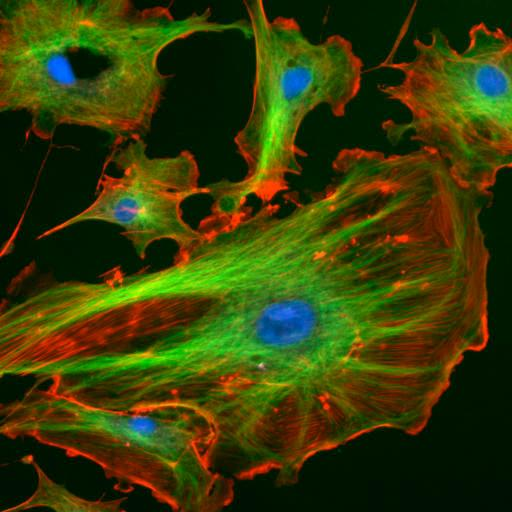
\includegraphics[height=0.3\textheight]{cell_mech} &
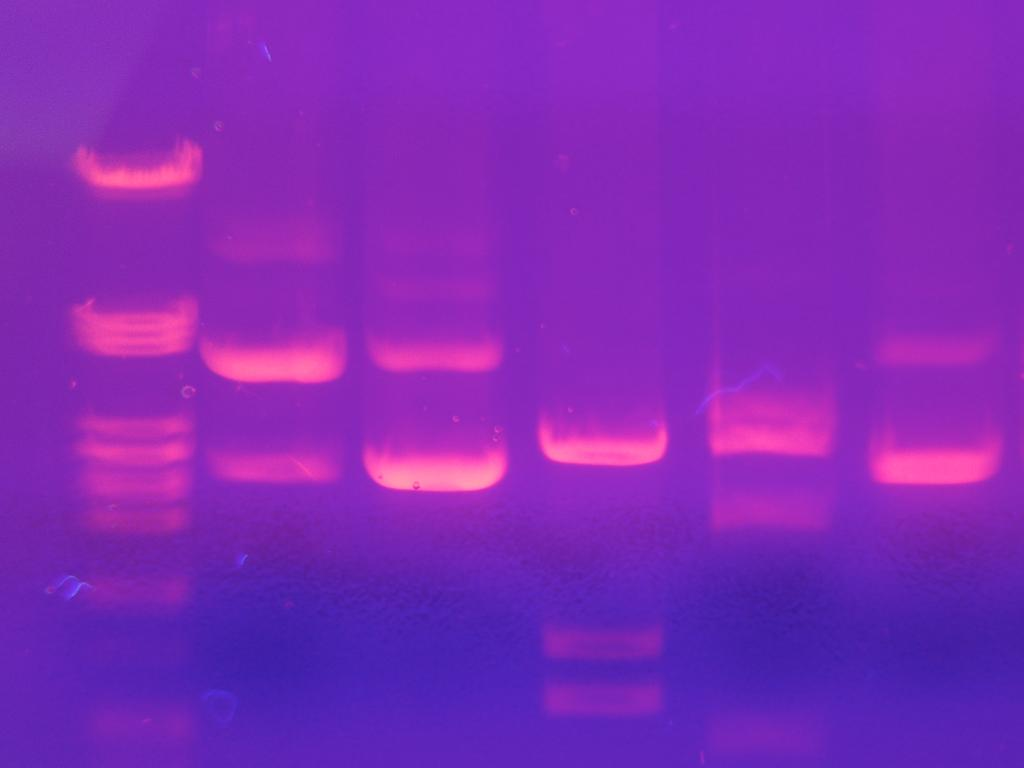
\includegraphics[height=0.3\textheight]{electrophoresis} &
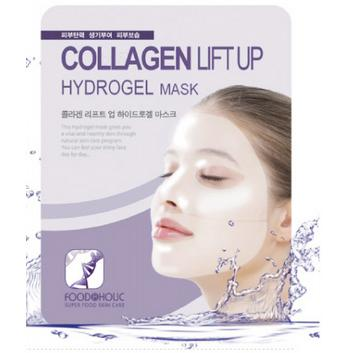
\includegraphics[height=0.3\textheight]{cosmetics} \\
Cell mechanics & Electrophoresis & Cosmetics\\
\end{tabu}
\begin{tabu}{X[c]X[c]}
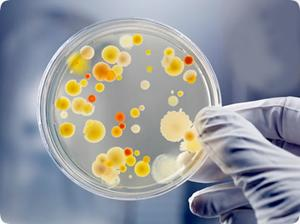
\includegraphics[height=0.3\textheight]{bacterial_culture} &
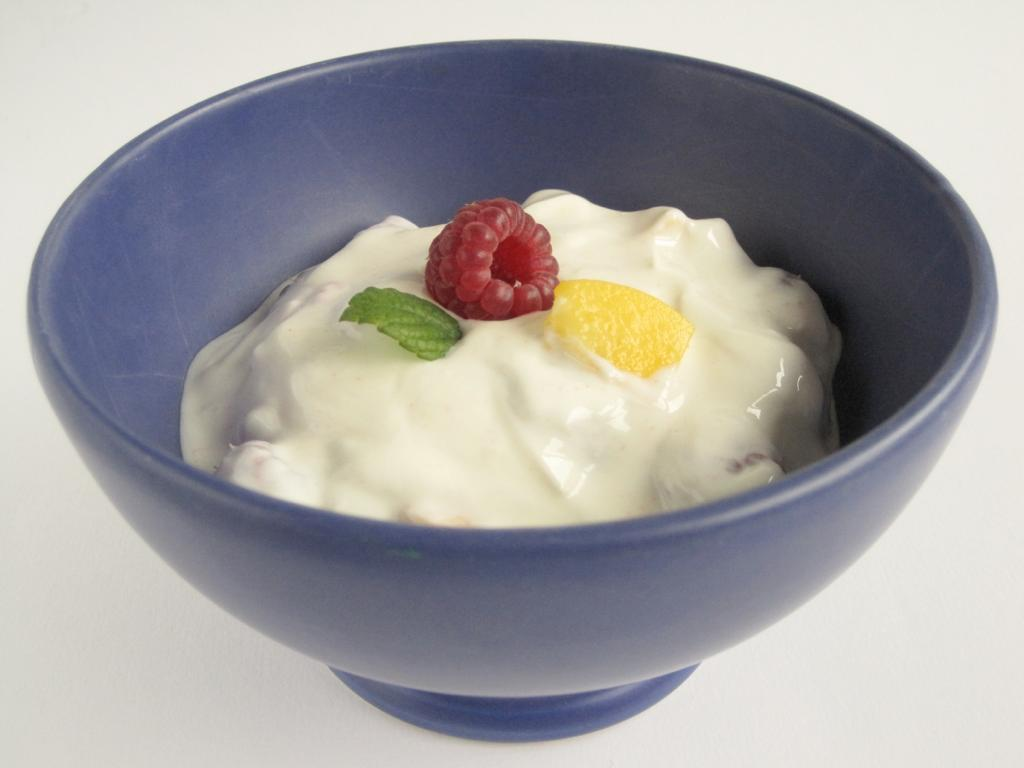
\includegraphics[height=0.3\textheight]{food} \\
Bacterial culture & Food\\
\end{tabu}

\begin{footnotesize}
\begin{block}{Sources}
\begin{tabu}{lXl}
Wikimedia Commons & www.madaboutscience.com & www.keautystore.com\\
\end{tabu}
\end{block}
\end{footnotesize}
\end{frame}



\begin{frame}{Fundamental issues in biogels}
\begin{itemize}
\item Linear elasticity is not well understood \textit{\scriptsize Gardel et al. Science 2004}
\item Strain and stress stiffening \textit{\scriptsize Storm et al. Nature 2005}
\item Fractures \textit{\scriptsize Bonn et al. Science 1998, Baumberger et al. Nature Material 2006}
\item Mechanical instabilities and morphogenesis \textit{\scriptsize Shyer et al. Science 2013}
\end{itemize}
\begin{tabu}{X[c]X[c]}
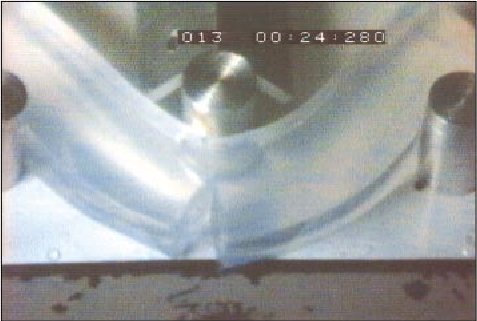
\includegraphics[height=6\baselineskip]{Bonn_fracture} &
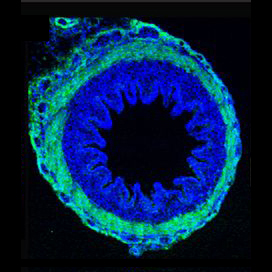
\includegraphics[height=6\baselineskip]{Villi_sq}
\end{tabu}
\begin{block}{Our questions}
\begin{itemize}
\item What is the behaviour of a biogel under shear deep into the nonlinear regime?
\item What is the role of the solvent in mechanical instabilities?
\end{itemize}
\end{block}
\end{frame}

%\section{Our system: Yoghurt}


%\tikzset{external/force remake}
\begin{frame}{Acid-set protein gel (Yoghurt)}
\begin{block}{Recipe: take your time}
\begin{itemize}
\item Water (\SI{30}{\celsius})
\item Sodium caseinate (milk protein) 4\%
\raisebox{0.6\normalbaselineskip}[0pt][0pt]{$\left.\rule{0pt}{1.1\normalbaselineskip}\right\}$ stable solution}
\item Glucono-$\delta$-lactone (GDL) 1\% $\Rightarrow$ slow homogeneous acidification
\end{itemize}
\end{block}

\begin{columns}
\column{0.5\textwidth}
\begin{tikzpicture}
	\begin{groupplot}[%
		group style={
			group name=g, group size=1 by 2,
			xticklabels at=edge bottom,
			vertical sep=0,
			},
		%xmode=log,
		%xmin=1e2,xmax=3e5,
		xmin=0, xmax=20,
		scale only axis,
		width=\textwidth-4em,
		height=0.3\textwidth,
		extra tick style={grid=major},%
		ylabel absolute, every axis y label/.append style={anchor=base, yshift=-0.5em}
		]
	\nextgroupplot[
		ymin=0, ymax=7, ylabel={pH},
		extra y ticks={4.6}, extra y tick labels={},%
		]
	\addplot+[no marks,Accent2] table[x expr={\thisrowno{0}/3600}]{Y190_cas4_gdl1.pH};
	\draw[help lines] (axis cs:0,4.6) -- (axis cs:3.88,4.6) node[pos=1, above right, font=\scriptsize] {isoelectric point $pH\approx 4.6$}  -- (axis cs:3.88,0);
	

	\nextgroupplot[
		xlabel={time (\si{\hour})},
		ymin=0, ylabel={$\textcolor{Accent2}{G^\prime}, \textcolor{Main}{G^{\prime\prime}}$ (\si{\pascal})},
		extra x ticks={17}, extra x tick labels={},
		]
	\addplot+[no marks,Accent2] table[x expr={\thisrowno{0}/3600}]{cas4_GDL1_Y22.prise};
	\addplot+[no marks,Main] table[x expr={\thisrowno{0}/3600}, y index=2]{cas4_GDL1_Y22.prise};
	\begin{scope}[font=\scriptsize]
		%\node[above right] at (rel axis cs:0,0) {casein ``micelles''};
		%\draw[<-] (axis cs:3.88,654) -- +(1em,0) node[right] {gelation};
		\node[anchor=base,rotate=80] at (axis cs:2.5,400) {gelation};
	\end{scope}
	\end{groupplot}
	\draw[<-] (g c1r2.south west) ++(0.5em,0) -- +(0,-1em) node[below,font=\footnotesize] {casein ``micelles''};
\end{tikzpicture}

\column{0.5\textwidth}
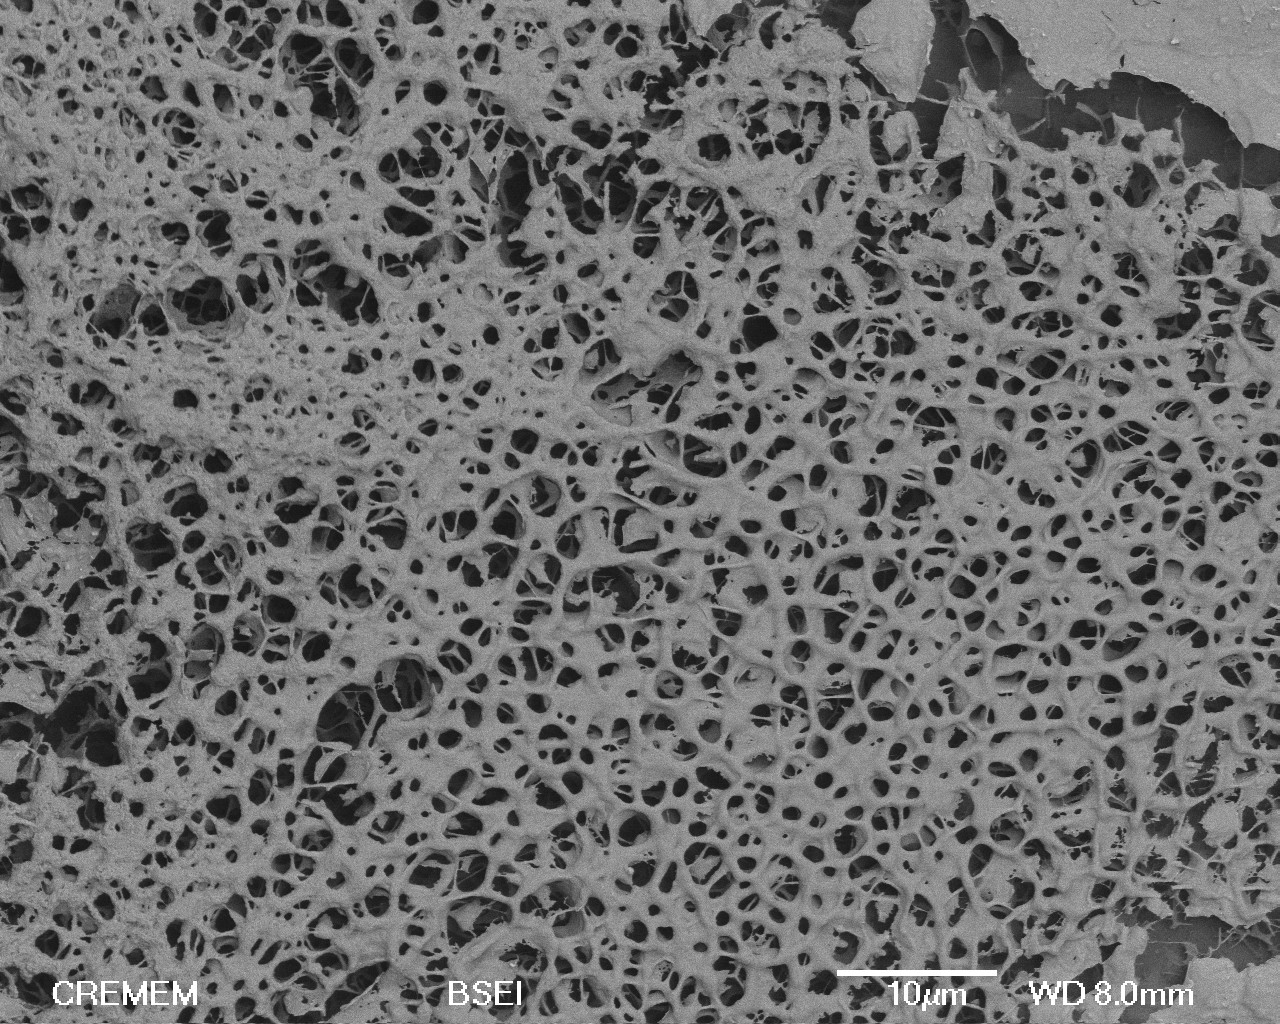
\includegraphics[width=\textwidth, clip=true, trim=0 0 0 10cm]{MEB_cas4_gdl1_22}

\begin{scriptsize}
\textit{Kaláb (1983),\linebreak Roefs \& van Vliet (1990),\linebreak Lucey \& Singh (1998)}
\end{scriptsize}
\end{columns}
\end{frame}
\tikzset{external/force remake=false}

\begin{frame}{Linear rheology: Power law (visco)elastic solid}
\[\text{stress}\rightarrow \sigma = G \gamma\leftarrow\text{strain}\]
\[\textcolor{Accent1}{\text{storage}\rightarrow} G^\prime + \imath G^{\prime\prime} \textcolor{Accent2}{\leftarrow\text{loss}}\]
\begin{tikzpicture}
\begin{loglogaxis}[
	height=0.8\textheight,
	width=\textwidth,
	xlabel={Frequency (\si{\hertz})}, ylabel={\textcolor{Accent1}{Storage} and \textcolor{Accent2}{loss} moduli (\si{\pascal})},
	domain={6e-2:70},
	]
	\addplot[Accent1, only marks, mark=*] table{freqsweep_Y265_cas4_GDL1.txt};
	\addplot[Accent2, only marks, mark=o] table[y=LossModulus]{freqsweep_Y265_cas4_GDL1.txt};
	\addplot[Main, no marks]{300*x^0.15}  node[midway, below right] {$G^\prime\sim G^{\prime\prime}\sim f^{0.15}$};
%	\addplot+[only marks, mark=*, forget plot] table{freqsweep_Y265_cas4_GDL1.txt} node[anchor=base east] {1\%};
%	\addplot+[only marks, mark=o, forget plot] table[y=LossModulus]{freqsweep_Y265_cas4_GDL1.txt} node[anchor=base east] {1\%};
%	\addplot{590*x^0.14};
%	\addplot+[only marks, mark=*, forget plot] table{freqsweep_Y277_cas4_GDL1.25.txt} node[anchor=base east] {1.25\%};
%	\addplot+[only marks, mark=o, forget plot] table[y=LossModulus]{freqsweep_Y277_cas4_GDL1.25.txt} node[anchor=base east] {1.25\%};
%	\addplot{350*x^0.12};
%	\addplot+[only marks, mark=*, forget plot] table{freqsweep_Y275_cas4_GDL1.5.txt} node[anchor=base east] {1.5\%};
%	\addplot+[only marks, mark=o, forget plot] table[y=LossModulus]{freqsweep_Y275_cas4_GDL1.5.txt} node[anchor=base east] {1.5\%};
%	\addplot{246*x^0.1};
%	\addplot+[only marks, mark=*, forget plot] table{freqsweep_Y268_cas4_GDL2.txt} node[anchor=base east] {2\%};
%	\addplot+[only marks, mark=o, forget plot] table[y=LossModulus]{freqsweep_Y268_cas4_GDL2.txt} node[anchor=base east] {2\%};
%	\addplot{163*x^0.067};
%	\addplot+[only marks, mark=*, forget plot] table{freqsweep_Y270_cas4_GDL3.txt} node[anchor=base east] {3\%};
%	\addplot+[only marks, mark=o, forget plot] table[y=LossModulus]{freqsweep_Y270_cas4_GDL3.txt} node[anchor=base east] {3\%};
%	\addplot{109*x^0.044};
%	\addplot+[only marks, mark=*, forget plot] table{freqsweep_Y271_cas4_GDL4.txt} node[anchor=base east] {4\%};
%	\addplot+[only marks, mark=o, forget plot] table[y=LossModulus]{freqsweep_Y271_cas4_GDL4.txt} node[anchor=base east] {4\%};
%	\addplot{76*x^0.035};
	
\end{loglogaxis}
\end{tikzpicture}
\end{frame}





\section*{Creep and yielding}

%\tikzset{external/force remake}
\begin{frame}{The yoghurt creep experiment}
\tikzsetnextfilename{creep_spoon}
\begin{tikzpicture}
\node[anchor=south west] (webcam){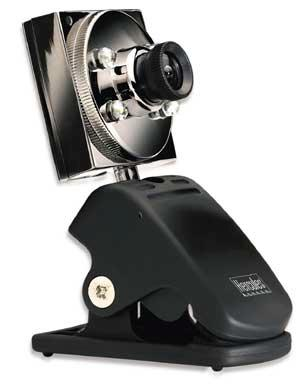
\includegraphics[width=0.2\textwidth]{webcam}};
\node[anchor=south] at (0.4\textwidth,0) (spoon) {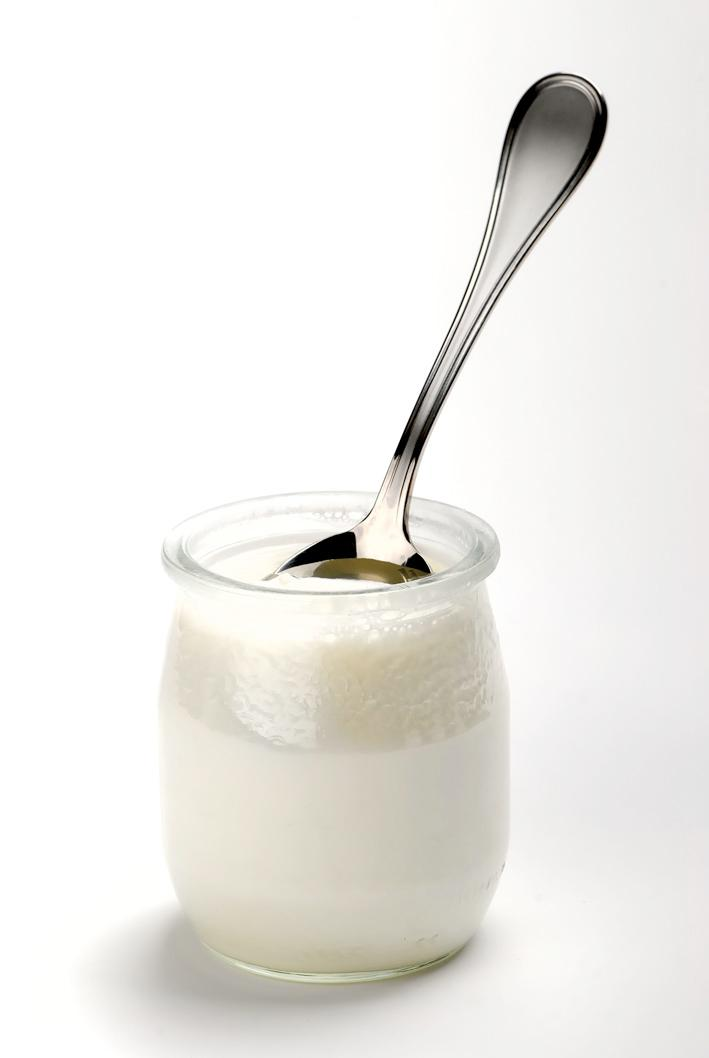
\includegraphics[width=0.3\textwidth]{spoon}};
\node[anchor=south east] at (\textwidth,0) (ultrasound) {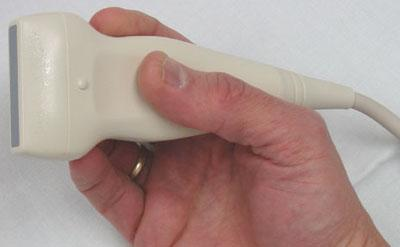
\includegraphics[width=0.4\textwidth]{ultrasound}};

\node[anchor=south west] at ($(ultrasound.north west)+(0,2em)$) (rheometer) {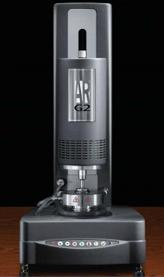
\includegraphics[height=0.4\textheight]{rheometer}};

\begin{scope}[draw]
	\node[below=0of spoon.south] (couette) {A Taylor-Couette cell where the yogurt is made \emph{in situ}};
	\draw[->] (couette) -- ($(spoon.south)+(0,2em)$);
	\node[above=0of ultrasound] {ultrasonic imaging};
	\node[above=0of webcam, text width=0.2\textwidth, align=center] {optical imaging};
	\draw[->] (spoon.north east) +(235:2em) -- (rheometer);
	\node[right=0of rheometer, text width=0.2\textwidth, align=center] {A rheometer imposes a constant stress $\sigma$ and records the strain $\gamma(t)$};
\end{scope}
\end{tikzpicture}
\end{frame}

%\tikzset{external/force remake}
\begin{frame}{The yoghurt creep experiment}
\movie[externalviewer]{\tikzsetnextfilename{creep_xp}\begin{tikzpicture}
\node[inner sep=0] (a) {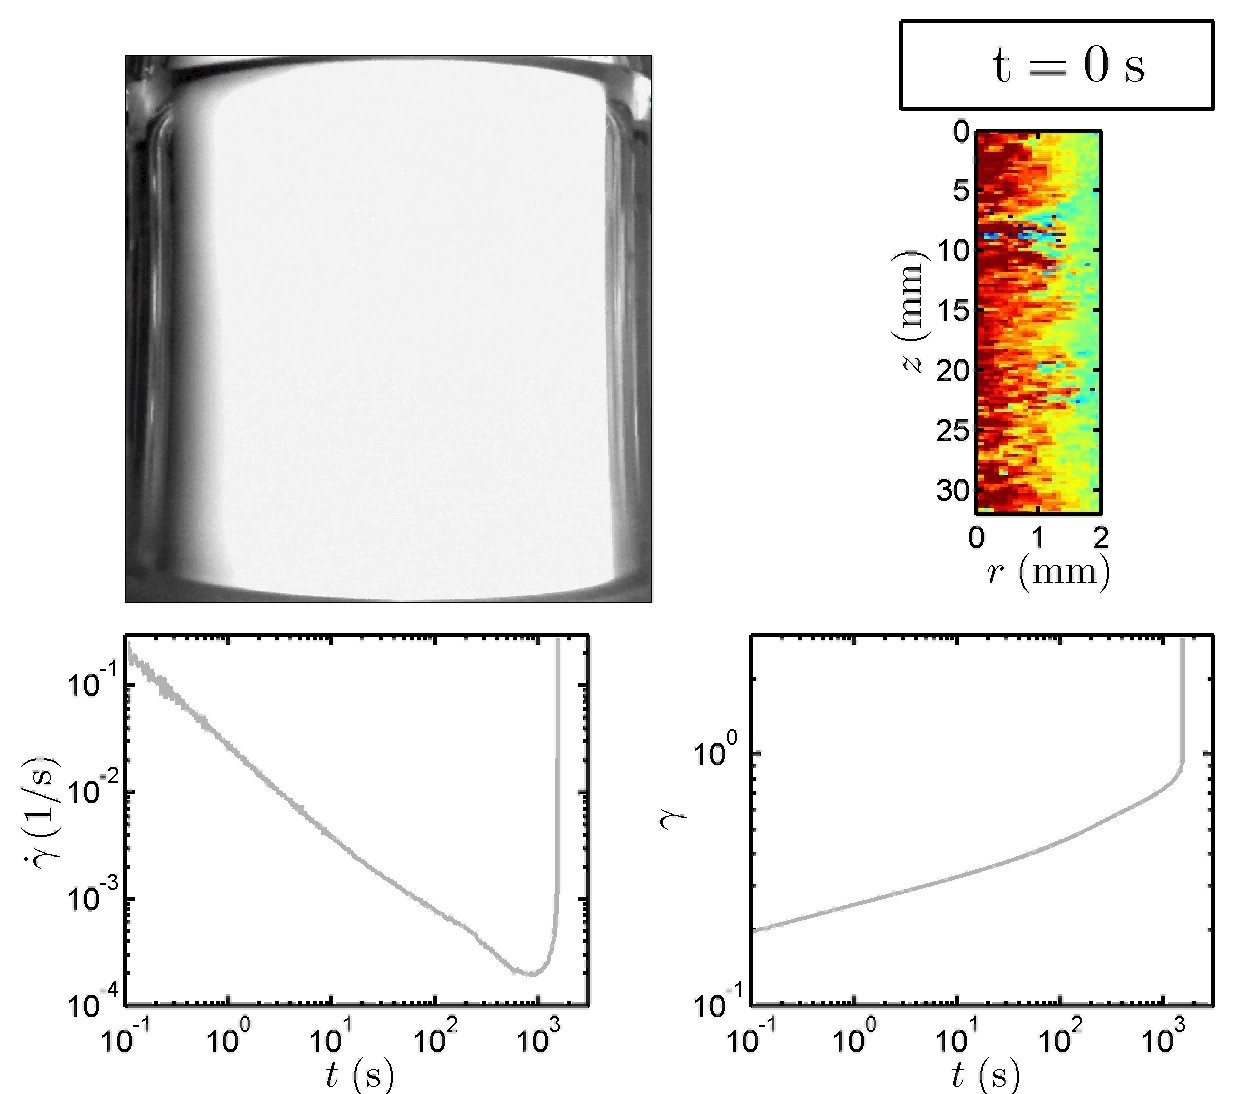
\includegraphics[height=16\baselineskip]{creep_experiment.jpg}};
\node[below right=\baselineskip of a.north east, inner sep=0] (vmap) {
\includegraphics[width=4\baselineskip]{jet_cmap}};

\begin{scope}[font=\footnotesize]
	\node[above=0 of vmap] {velocity map};
	\node[below=0 of vmap.south west] {-50};
	\node[below=0 of vmap.south] (v0) {0};
	\node[below=0 of vmap.south east] {50};
	\node[below=0 of v0, inner sep=0]{\si{\micro\metre\per\second}};
\end{scope}

\begin{scope}[shift={(a.north west)}, shift={(5.8\baselineskip,-1.1\baselineskip)}, ultra thick]
	\draw[Accent1, x radius=3.1\baselineskip, y radius=0.3\baselineskip] ellipse[] ++(3.1\baselineskip,0)  -- ++(0,-7.4\baselineskip)  ++(-3.1\baselineskip,0) ellipse[] ++(-3.1\baselineskip,0)  -- ++(0,7.4\baselineskip);
	\shadedraw[Accent2,ball color=Accent2, x radius=2\baselineskip, y radius=0.1\baselineskip] ellipse[] ++(2\baselineskip,0)  -- ++(0,-7.4\baselineskip)  ++(-2\baselineskip,0) ellipse[] ++(-2\baselineskip,0)  -- ++(0,7.4\baselineskip);
	\fill[Accent2, left color=black,right color=black, middle color=Accent2, ] (-0.3\baselineskip,0) rectangle +(0.6\baselineskip, \baselineskip);
	\begin{scope}[Main]
		\node[draw, minimum height=4.2\baselineskip, minimum width=1.5\baselineskip] at (2.5\baselineskip,-4\baselineskip) (window){};
		\node[draw, minimum height=7.2\baselineskip, minimum width=4\baselineskip] at (8.9\baselineskip,-4.2\baselineskip) (USV){};
		\draw(window.north east) -- (USV.north west) (window.south east) -- (USV.south west);
		\node[right, text width=4\baselineskip] at (USV.east) {ultrasound region of interest};
	\end{scope}

\draw[<->,thin] ++(-2\baselineskip,-\baselineskip) -- +(-1.1\baselineskip,0) node[midway,above] {\SI{2}{\milli\metre}};
\end{scope}
\draw[->] (window.north west) ++(-1em, 0.2em) -- +(1em,0) node[midway,above,inner sep=1pt] {$r$};
\draw[->] (window.north west) ++(-1em, 0.2em) -- +(0,-1em)  node[midway,left] {$z$};

\node[text width=4\baselineskip] at (-3\baselineskip,-2.5\baselineskip) {shear rate response};
\node at (5\baselineskip,-2.5\baselineskip) {strain response};
\end{tikzpicture}%
}{Yaourt141_enhanced.avi}
\end{frame}
%\tikzset{external/force remake=false}

\begin{frame}{The yoghurt creep experiment}
\includegraphics[width=\textwidth]{creep/Fig3}
\begin{center}\tikzsetnextfilename{creep_xp_snapshot}
\begin{tikzpicture}
\begin{groupplot}[
	group style={
		group name=g, group size=2 by 1,
		horizontal sep=4\baselineskip,
		},
	xmode=log,
	ymode=log,
	xlabel={$t$ (\si{\second})},
	xmin=0.1,
	%restrict x to domain=0.05:3e3,
	]
	\nextgroupplot[ylabel={strain rate $\dot\gamma$ (\si{\per\second})}, ymin=1e-4, ymax=2e-1]
	\addplot[Accent1] table {Y110_300Pa.gdot}; 
	\addplot[Accent2, only marks, mark=o] coordinates {(31, 1.6e-3) (889, 2e-4) (1442, 5.5e-4) (1509, 1.1e-2)};

	\nextgroupplot[
		ylabel={strain $\gamma$},ymin=0.16,ymax=2,
		ytick={0.2, 0.4,0.8,1.6}, yticklabels={0.2, 0.4,0.8,1.6},]
	\addplot[Accent1] table {Y110_300Pa.txt}; 
	\addplot[Accent2, only marks, mark=o] coordinates {(31, 0.37481) (880, 0.70529) (1459, 0.87393) (1526,0.93622)};

\end{groupplot}
\end{tikzpicture}
\end{center}
\end{frame}

\begin{frame}{Creep rheology: Three regimes}
\tikzsetnextfilename{three_regimes}
\begin{tikzpicture}
\begin{loglogaxis}[
   name=g,
	width=\textwidth,
	height=0.8\textheight,
	xmin=2e-2, xmax=4e5, xlabel={time (\si{\second})},
	ymin=0.2,ymax=2,
	ytick={0.2, 0.4,0.8,1.6}, yticklabels={0.2, 0.4,0.8,1.6},
	ylabel={strain $\gamma$},
	extra tick style={grid=major},%
	extra y ticks={1}, extra y tick labels={1.0},
	cycle list name=earthy,
	axis on top,
	]
	\fill[Accent1!20]
		(axis cs:10,0.4) ellipse[rotate=-30, x radius=0.2\textwidth, y radius=0.12\textwidth]
		(axis cs:2e2,1.6) ellipse[x radius=0.35\textwidth, y radius=0.05\textwidth]
		(axis cs:3e3,0.85) ellipse[rotate=-7.5, x radius=0.3\textwidth, y radius=0.07\textwidth]
		;
	\node[above right] at (axis cs:1e1,0.2) {primary};
	\node[below left] at (axis cs:4e5,0.7) {secondary};
	\node[left] at (axis cs:5,1.6) {tertiary};
	\addplot table{Y27_200Pa_gamma_decimated.txt} node (s200){};
	\addplot table{Y38_300Pa_gamma_decimated.txt} node (s300){};
	\addplot table{Y25_400Pa_gamma_decimated.txt}  node (s400){};
	\addplot table{Y32_550Pa_gamma_decimated.txt}  node (s550){};
	\addplot table{Y39_1000Pa_gamma_decimated.txt} node (s1000){};
\end{loglogaxis}
\begin{scope}[anchor=base, every node/.style={yshift=0.2em}]
	\node[red!40!black] at (s200 |- g.outer north) {\SI{200}{\pascal}};
	\node[red!60!black] at (s300 |- g.outer north) {300};
	\node[red!80!black] at (s400 |- g.outer north) {400};
	\node[red] at (s550 |- g.outer north) {550};
	\node[red!80!yellow] at (s1000 |- g.outer north) {1000};
\end{scope}
\end{tikzpicture}

Failure at $\gamma\approx 1$ for a well defined time $\tau_f$
\end{frame}

%\tikzset{external/force remake}
\begin{frame}{Failure time}
\begin{columns}
\column{0.55\textwidth}
\tikzsetnextfilename{basquin}
\begin{tikzpicture}
\begin{loglogaxis}[
	width=\textwidth,
	height=0.8\textwidth,
	xlabel={$\sigma$ (\si{\pascal})},
	ylabel={$\tau_f$ (\si{\second})},
	xmin=100, ymin=10, ymax=1e6,
	xtick={100, 200,..., 1000}, xticklabels={100, 200,,, 500,,,,, 1000},
	]
	\addplot[only marks, Accent1] table[y index=3]{creep_cas4_gdl1_MCR.txt};
	\addplot[no marks, black, domain={100:1000}] {4.2e17*x^(-5.45)} node [midway, above right] {$\tau_f\sim \sigma^{-5.5}$};
\end{loglogaxis}
\end{tikzpicture}

\begin{block}{Basquin law}
\begin{itemize}
\item fatigue (oscillatory stress)
\item heterogeneous solids
\item no yield stress
\end{itemize}
\end{block}

\column{0.45\textwidth}
\tikzsetnextfilename{basqun_otherfits}
\begin{tikzpicture}
\begin{groupplot}[
	group style={
		group name=g, group size=1 by 2,
		},
	width=\textwidth,
	height=0.7\textwidth,
	ymode=log,
	ylabel={$\tau_f$ (\si{\second})},
	ymin=10, ymax=1e6,
	]
	\nextgroupplot[
		xlabel={$\sigma$ (\si{\pascal})},
		xtick={200,600,1000},
		]
		\addplot[only marks, Accent1] table[y index=3]{creep_cas4_gdl1_MCR.txt};
		\addplot[no marks, black, domain={100:1000}] {6.5e5*exp(-x/84)} node [pos=0.25, above right] {$\tau_f\nsim e^{-\frac{\sigma}{\sigma_0}}$};
		
	\nextgroupplot[
		xlabel={$1/\sigma$ (\si{\per\pascal})},
		]
		\addplot[only marks, Accent1] table[x expr=1/\thisrowno{0}, y index=3]{creep_cas4_gdl1_MCR.txt};
		\addplot[no marks, black, domain={1e-3:7e-3}] {20.3*exp(1720*x)} node [pos=0.25, below right] {$\tau_f\nsim e^\frac{\sigma_0}{\sigma}$};
\end{groupplot}
\end{tikzpicture}

Activated processes unlikely (Eyring, Griffith, Taylor, \ldots)
\end{columns}
\end{frame}

%\tikzset{external/force remake}
\begin{frame}{Primary creep}
\begin{columns}
\column{0.55\textwidth}
\tikzsetnextfilename{primary_creep}
\begin{tikzpicture}
\begin{loglogaxis}[
	name=g,
	width=\textwidth,
	height=0.8\textwidth,
	xmin=2e-2, xmax=4e5, xlabel={time (\si{\second})},
	ylabel={Strain rate $\dot{\gamma}$ (\si{\per\second})},
	cycle list name=earthy,
	no marks,
	]
	\addplot table[y index=2]{Y27_200Pa_gdot_decimated.txt} node (s200){};
	\addplot table[y index=2]{Y38_300Pa_gdot_decimated.txt} node (s300){};
	\addplot table[y index=2]{Y25_400Pa_gdot_decimated.txt}  node (s400){};
	\addplot table[y index=2]{Y32_550Pa_gdot_decimated.txt}  node (s550){};
	\addplot table[y index=2]{Y39_1000Pa_gdot_decimated.txt} node (s1000){};
	\addplot[Accent2, ultra thick, domain={0.1:1e3}] {0.01*x^(-0.85)} node[pos=0.75, below left] {$\dot{\gamma}(t)\sim t^{-0.85}$};
\end{loglogaxis}
\begin{scope}[anchor=base east, every node/.style={ rotate=90}]
	\node[red!40!black] at (s200 |- g.outer north) {\SI{200}{\pascal}};
	\node[red!60!black] at (s300 |- g.outer north) {300};
	\node[red!80!black] at (s400 |- g.outer north) {400};
	\node[red] at (s550 |- g.outer north) {550};
	\node[red!80!yellow] at (s1000 |- g.outer north) {1000};
\end{scope}
\end{tikzpicture}

\begin{block}{Primary creep $\Rightarrow$ ``Andrade'' creep}
Power-law creep known in \alert{solids} for over a century

Classically explained by disinclination dynamics in crystals
\end{block}

\column{0.45\textwidth}
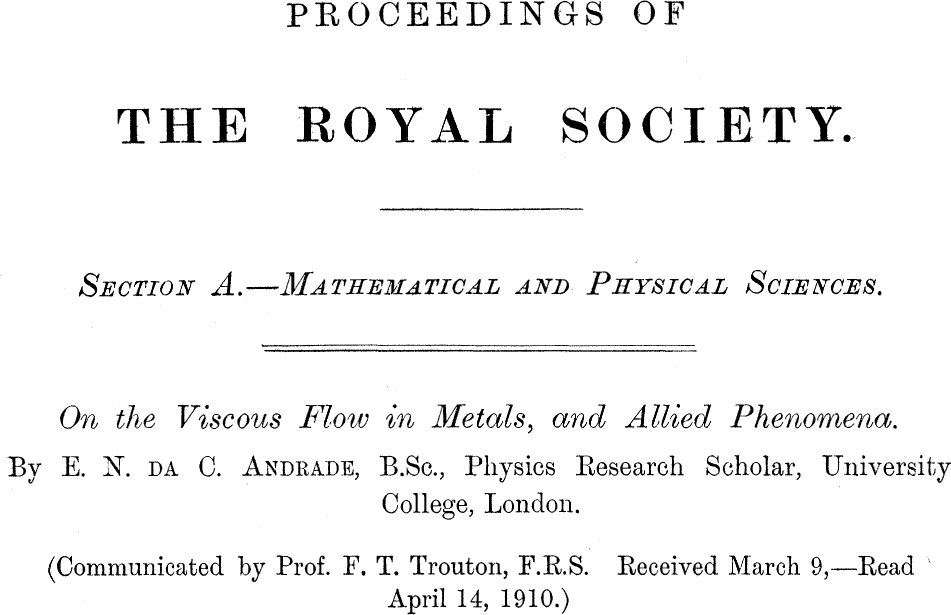
\includegraphics[width=\textwidth]{Andrade_1910}

\bigskip
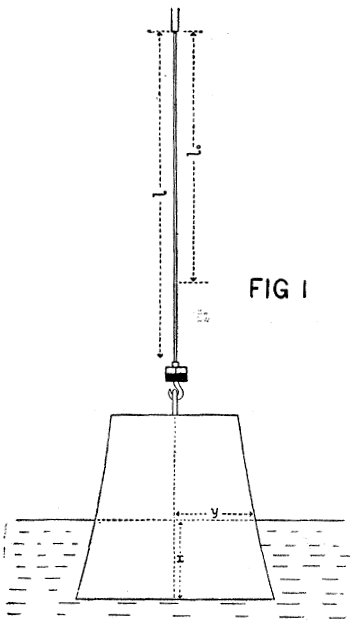
\includegraphics[height=7\baselineskip]{Andrade_1910_fig1}%
\tikzsetnextfilename{Andrade_historical}%
\begin{tikzpicture}
\node[inner sep=0] (a){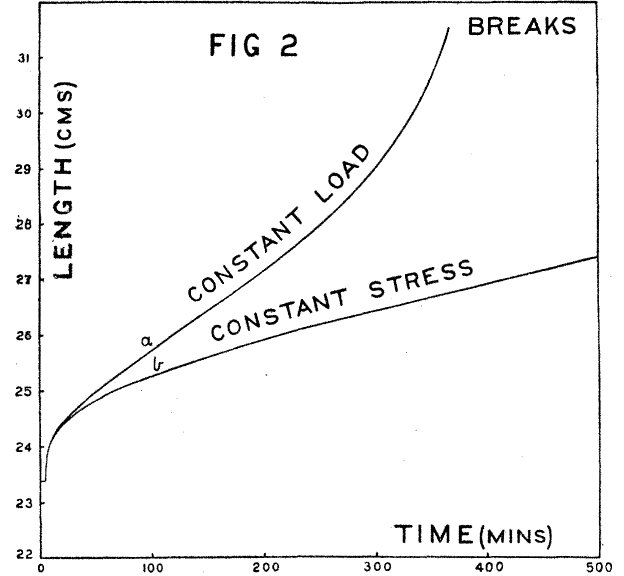
\includegraphics[height=7\baselineskip]{Andrade_1910_fig2}};
\node[below right=0 and 1em of a.north west, font=\footnotesize,fill=white] {lead \& copper};
\node[above left=1em of a.south east, Accent2] {$\gamma-\gamma_0 \sim t^{1/3}$};
\end{tikzpicture}
\end{columns}
\end{frame}


%\tikzset{external/force remake}
\begin{frame}{Primary creep}
\begin{block}{Local insight from \movie[externalviewer]{ultrasounds}{Yaourt110_primary.avi}}
\begin{itemize}
	\item homogeneous \movie[externalviewer]{strain field}{Yaourt110_profils.avi} (no wall slip, no shear band)
	\item if present, plastic events are below our resolution (a few \si{\micro\metre})
\end{itemize}
\end{block}

\begin{block}{Partial creep and recovery}
\tikzsetnextfilename{recovery}
\begin{tikzpicture}
\begin{axis}[
	width=\textwidth,
	height=8\baselineskip,
	xlabel={time (\si{\hour})},
	ylabel={strain $\gamma$},
	xmin=-0.15, xmax=7.5, xtick={0, 1, ..., 7},
	axis background/.style={fill=white},
	]
	\addplot[black, no marks] table[x expr={\thisrowno{0}/3600}] {Y261_oscil_creep_recovery_100Pa_decimated.txt};
	\begin{scope}[<-,Main, inner sep=0]
	\draw (axis cs:0,0) -- +(1em,0) node[anchor=west]{$\sigma\leftarrow \SI{100}{\pascal}$};
	\draw (axis cs:1/6,0.2727007) -- +(1em,0) node[anchor=west]{$\sigma\leftarrow 0$};
	\draw (axis cs:2.388,0.0159) -- +(0,1em) node[anchor=base east]{$\gamma\leftarrow 0$};
	\end{scope}
\end{axis}
\end{tikzpicture}
\end{block}

$\Rightarrow$ Primary creep is ``kinetically'' reversible (no detectable structure damage, but viscous dissipation)
\end{frame}




%\tikzset{external/force remake}
\begin{frame}{Dimensionless creep response}
\begin{columns}
\column{0.55\textwidth}
\tikzsetnextfilename{primary_rescaled}
\begin{tikzpicture}
\begin{loglogaxis}[
	width=\textwidth,
	height=0.8\textwidth,
	xmin=1e-5, xmax=2, xlabel={$t/\tau_f$},
	ylabel={$\dot{\gamma}/\dot{\gamma}_\text{min}$},
	cycle list name=earthy,
	clip mode=individual,
	]
	\addplot table[x index=1, y index=3]{Y27_200Pa_gdot_decimated.txt} node (s200){};
	\addplot table[x index=1, y index=3]{Y38_300Pa_gdot_decimated.txt} node (s300){};
	\addplot table[x index=1, y index=3]{Y25_400Pa_gdot_decimated.txt}  node (s400){};
	\addplot table[x index=1, y index=3]{Y32_550Pa_gdot_decimated.txt}  node (s550){};
	\addplot table[x index=1, y index=3]{Y39_1000Pa_gdot_decimated.txt} node (s1000){};
	\addplot[yellow, ultra thick, domain={1e-4:0.1}] {0.378*x^(-0.85)} node[Accent2,pos=0.75, below left] {$\frac{\dot{\gamma}(t)}{\dot{\gamma}_\text{min}}\sim \left(\frac{t}{\tau_f}\right)^{-0.85}$};
\end{loglogaxis}
\end{tikzpicture}

Linear viscoelasticity accounts for the Andrade exponent

\column{0.45\textwidth}
\tikzsetnextfilename{linear_rheology}
\begin{tikzpicture}
\begin{loglogaxis}[
	height=0.8\textwidth,
	width=\textwidth,
	xlabel={Frequency (\si{\hertz})}, ylabel={\textcolor{Accent1}{$G^\prime$}, \textcolor{Accent2}{$G^{\prime\prime}$}(\si{\pascal})},
	domain={6e-2:70},
	ymin=10,
	]
	\addplot[Accent1, only marks, mark=*] table{freqsweep_Y265_cas4_GDL1.txt};
	\addplot[Accent2, only marks, mark=o] table[y=LossModulus]{freqsweep_Y265_cas4_GDL1.txt};
	\addplot[Main, no marks]{100*x^0.15}  node[midway, below=1em] {$G^\prime\sim G^{\prime\prime}\sim f^{0.15}$};
	
\end{loglogaxis}
\end{tikzpicture}
\textcolor{Main}{
\begin{align*}
\Rightarrow & J(t) \equiv& \frac{\gamma(t)}{\sigma}\sim& t^{0.15}\\
\Rightarrow & \dot{\gamma}(t)\sim& t^{0.15-1} =& t^{-0.85}
\end{align*}
}
\end{columns}
\end{frame}

%\tikzset{external/force remake}
\begin{frame}{Tertiary creep}
\begin{columns}
\column{0.55\textwidth}
Time to failure

\tikzsetnextfilename{tertiary_rescaled}
\begin{tikzpicture}
\begin{loglogaxis}[
	width=\textwidth,
	height=0.8\textwidth,
	xmin=1e-5, xmax=2, xlabel={$(\tau_f-t)/\tau_f$},
	x dir=reverse,
	ylabel={$\dot{\gamma}/\dot{\gamma}_\text{min}$},
	cycle list name=earthy,
	clip mode=individual,
	]
	\addplot table[x expr=1-\thisrowno{1}, y index=3]{Y27_200Pa_gdot_decimated.txt} node (s200){};
	\addplot table[x expr=1-\thisrowno{1}, y index=3]{Y38_300Pa_gdot_decimated.txt} node (s300){};
	\addplot table[x expr=1-\thisrowno{1}, y index=3]{Y25_400Pa_gdot_decimated.txt}  node (s400){};
	\addplot table[x expr=1-\thisrowno{1}, y index=3]{Y32_550Pa_gdot_decimated.txt}  node (s550){};
	\addplot table[x expr=1-\thisrowno{1}, y index=3]{Y39_1000Pa_gdot_decimated.txt} node (s1000){};
	\addplot[yellow, ultra thick, domain={1e-4:0.1}] {0.187/x} node[Accent2, pos=0.6, below right, inner sep=0] {$\frac{\dot{\gamma}(t)}{\dot{\gamma}_\text{min}}\sim \left(\frac{\tau_f}{\tau_f-t}\right)$};
\end{loglogaxis}
\end{tikzpicture}

Close to failure: 
\begin{itemize}
\item finite time singularity
\item logarithmic divergence
\end{itemize}
$\Rightarrow$ dominated by fracture growth

\column{0.45\textwidth}
\begin{block}{Fracture growth}
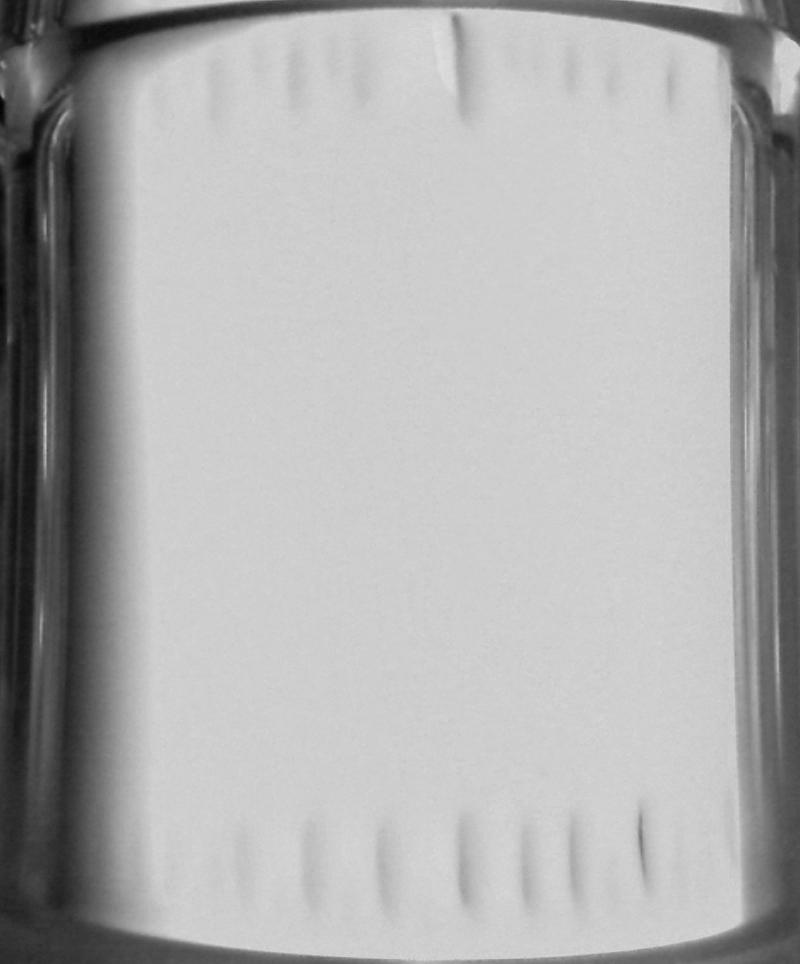
\includegraphics[width=0.33\textwidth]{Y110_2013-03-01_03-15-00.jpg}\hfill
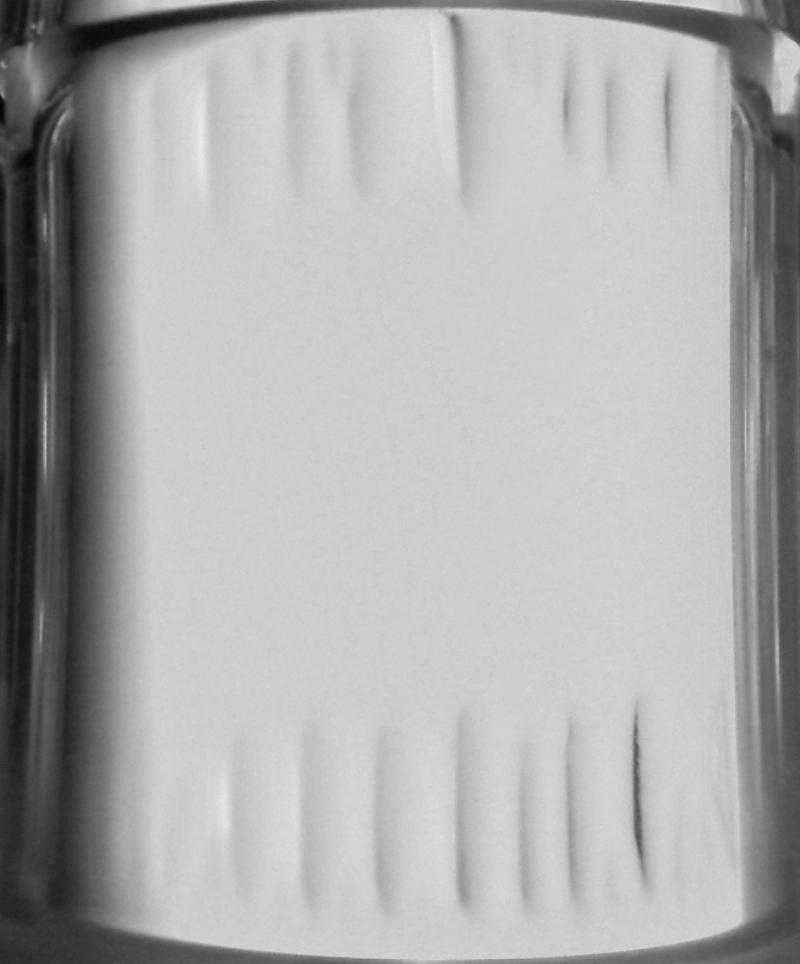
\includegraphics[width=0.33\textwidth]{Y110_2013-03-01_03-20-00.jpg}\hfill
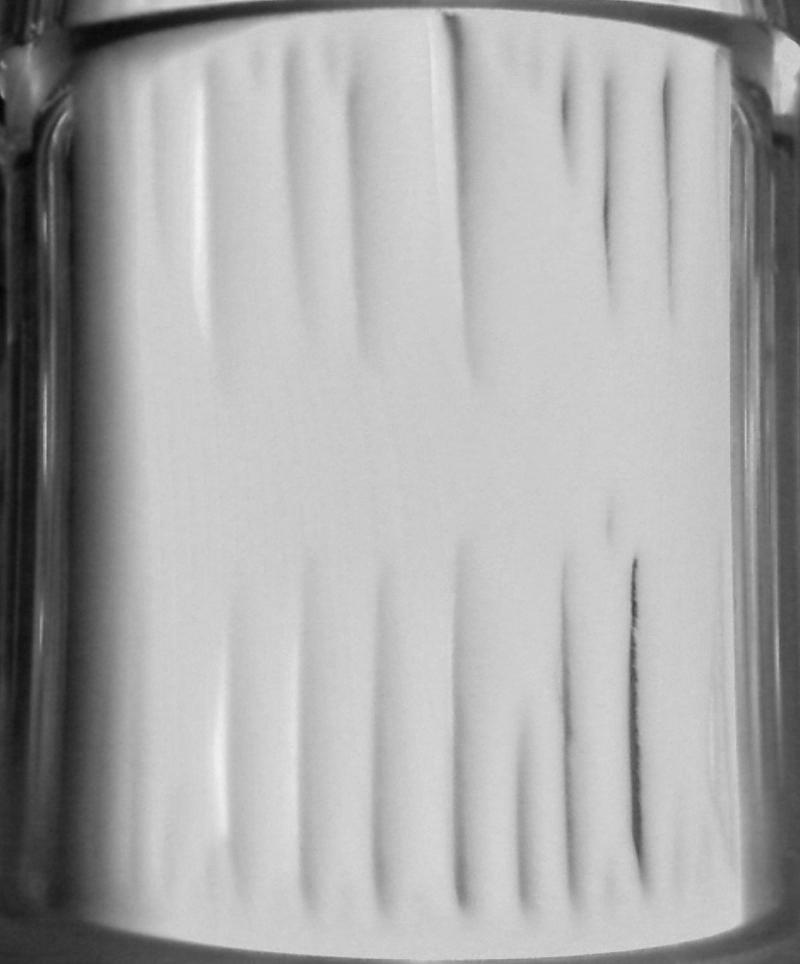
\includegraphics[width=0.33\textwidth]{Y110_2013-03-01_03-21-15.jpg}

\tikzsetnextfilename{fracture_length}
\begin{tikzpicture}
\begin{axis}[
	width=\textwidth,
	height=0.8\textwidth,
	xmin=1e-3, xmax=1, xlabel={$(\tau_f-t)/\tau_f$},
	xmode=log, x dir=reverse,
	ylabel={$\ell/H$},
	ymin=0, ymax=0.5,
	clip mode=individual,
	axis background/.style={fill=white},
	]
	\addplot[only marks, Accent1, error bars/.cd, y dir=both, y explicit] table[y error index=2]{Y110_fracturelength.txt};
	\addplot[Accent2, ultra thick, no marks, domain={1e-3:1}] {- 0.06 * ln(x)} node [pos=0.25,left=1em] {$\frac{\ell}{H}\sim \ln\frac{\tau_f-t}{\tau_f}$};
\end{axis}
\end{tikzpicture}
\end{block}
\end{columns}
\end{frame}

%\tikzset{external/force remake}
\begin{frame}{Secondary creep: a crossover}
\begin{columns}
\column{0.55\textwidth}
Creep responses in linear scales

\tikzsetnextfilename{secondary_rescaled}
\begin{tikzpicture}
\begin{axis}[
	width=\textwidth,
	height=0.8\textwidth,
	xmin=0, xmax=1, xlabel={$t/\tau_f$},
	ylabel={$\dot{\gamma}/\dot{\gamma}_\text{min}$},
	ymin=0.5, ymax=4,
	cycle list name=earthy,
	restrict y to domain=0.5:10,
	clip mode=individual,
	]
	\addplot table[x index=1, y index=3]{Y27_200Pa_gdot_decimated.txt} node (s200){};
	\addplot table[x index=1, y index=3]{Y38_300Pa_gdot_decimated.txt} node (s300){};
	\addplot table[x index=1, y index=3]{Y25_400Pa_gdot_decimated.txt}  node (s400){};
	\addplot table[x index=1, y index=3]{Y32_550Pa_gdot_decimated.txt}  node (s550){};
	\addplot table[x index=1, y index=3]{Y39_1000Pa_gdot_decimated.txt} node (s1000){};
	\addplot[yellow, ultra thick, domain={0.01:0.99}] {0.378*x^(-0.85) + 0.187/(1-x)};
	\draw[<-] (axis cs:0.56,1) -- +(0,1em) node[above] {$\tau_\text{min}$};
\end{axis}
\end{tikzpicture}
\begin{block}{Master curve}
\[\frac{\dot{\gamma}(t)}{\dot{\gamma}_\text{min}} = \underbrace{\lambda \left(\frac{t}{\tau_f}\right)^{-0.85}}_\text{Andrade} + \underbrace{\frac{\mu}{1 - t/\tau_f}}_\text{fractures}\]
\end{block}


\column{0.45\textwidth}
\structure{Monkman-Grant relation}
\tikzsetnextfilename{Monkman-Grant}
\begin{tikzpicture}
\begin{loglogaxis}[
	width=\textwidth,
	height=0.8\textwidth,
	xlabel={$\tau_f$ (\si{\second})},
	ylabel={$\tau_\text{min}$ (\si{\second})},
	xmin=10, xmax=1e6, ymin=10, ymax=1e6,
	]
	\addplot[only marks, Accent1] table[x index=3, y index=4]{creep_cas4_gdl1_MCR.txt};
	\addplot[no marks, black, domain={10:1e6}] {0.56*x)};
\end{loglogaxis}
\end{tikzpicture}
\[\tau_\text{min} \approx 0.6 \tau_f\]
``Early time'' response allows to predict failure time
\end{columns}
\end{frame}

\begin{frame}{What about theories and models?}
\begin{columns}
\column{0.35\textwidth}
\begin{block}{Discrete dislocation dynamics (dense)}
\textit{\footnotesize Miguel et al., PRL 2002}

\hspace{1em}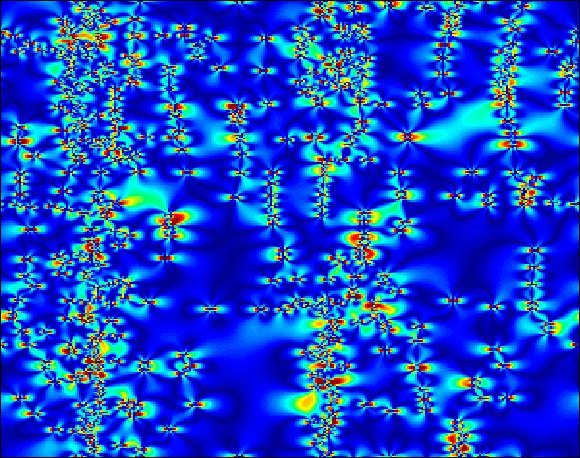
\includegraphics[width=\textwidth-2em]{Miguel_2002_img}

\medskip
\hspace{1em}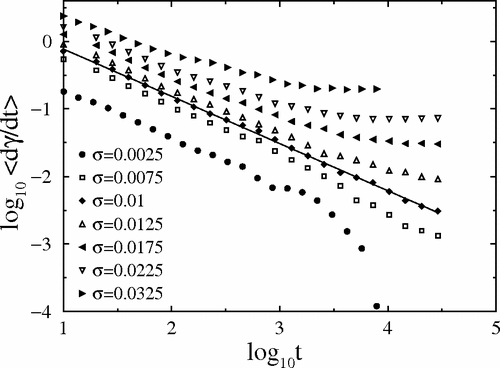
\includegraphics[width=\textwidth-2em]{Miguel_2002_graph}

predicts Andrade creep \alert{but} no fracture
\end{block}
\column{0.65\textwidth}
\begin{columns}
\column{0.5\textwidth+1em}
\structure{Fibre bundle model~\#1}

\textit{\footnotesize Jagla et al., PRE 2011}
\begin{itemize}
\item elastic fibres
\item local yield strain
\item local coupling
\end{itemize}

\hspace{1em}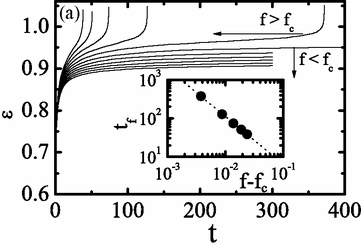
\includegraphics[width=\textwidth-1em]{Jagla_2011_gamma}
\[\tau_f\sim\left(\sigma-\alert{\sigma_c}\right)^{-1.25}\]

\column{0.5\textwidth-1em}
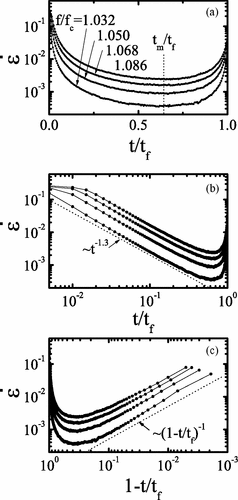
\includegraphics[width=\textwidth]{Jagla_2011_3regimes}
\end{columns}
predicts Andrade creep and failure \alert{but} critical stress
\end{columns}
\end{frame}


\begin{frame}{What about theories and models?}
\structure{Fibre bundle model~\#2}

elastic fibres + local yield strain + damage accumulation
\begin{block}{\textit{\footnotesize Kun et al. J. Stat Mech 2006, PRL 2008}}
\begin{columns}
\column{0.7\textwidth}
\tikzsetnextfilename{Kun_2006_basquin}
\begin{tikzpicture}[inner sep=0]
\node(a){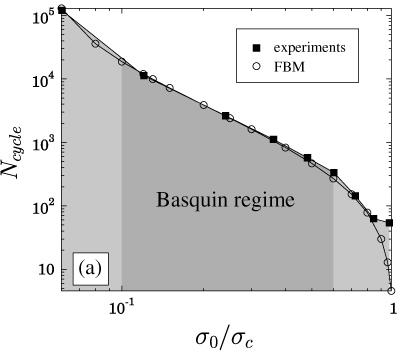
\includegraphics[height=5\baselineskip]{Kun_2006_basquin.png}};
\node[fill=white,yshift=-0.5em] at (a) {$\tau_f \sim \sigma^{-\beta}$};
\end{tikzpicture}\,
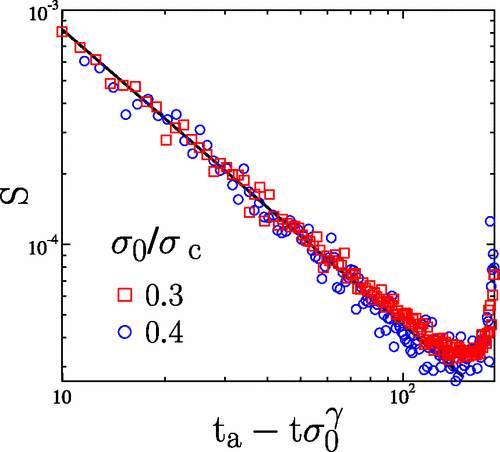
\includegraphics[height=5\baselineskip]{Kun_2008_Basquin}\,
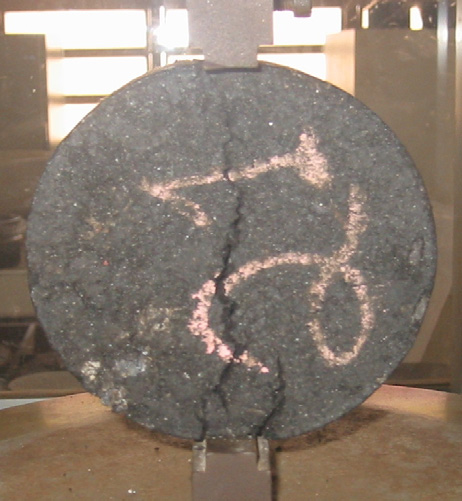
\includegraphics[height=5\baselineskip]{asphalt}
\column{0.3\textwidth}
$\beta$ exponent of damage accumulation
\[\dot{\gamma}\sim \left(\tau_f-t\right)^{-1/(1+\beta)}\]
\end{columns}
\end{block}

\begin{columns}
\column{0.65\textwidth}
\begin{block}{\textit{\footnotesize Halász et al., PRE 2012}}
\tikzsetnextfilename{Halasz}
\begin{tikzpicture}[inner sep=0, ultra thick, font=\footnotesize]
\node (g) {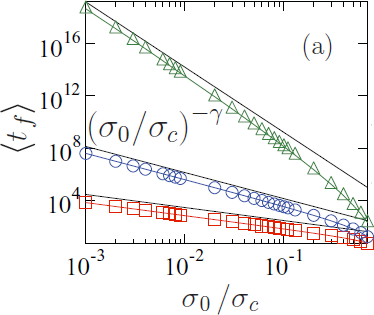
\includegraphics[height=7\baselineskip]{Halasz_2012_Basquin}};
\node[draw=green!50!black, below right=0 and \baselineskip of g.north east] (c) {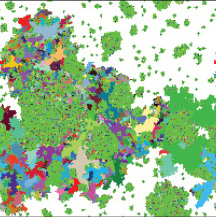
\includegraphics[height=4\baselineskip]{Halasz_2012_crack}};
\node[draw=red, above right=0 and 6\baselineskip of g.south east] (d) {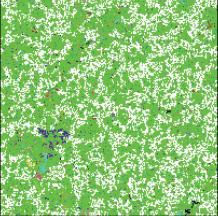
\includegraphics[height=4\baselineskip]{Halasz_2012_disordered}};
\draw[->,green!50!black] (c.west) -- ++(-2\baselineskip,0) node[above] {$\beta=5$} node[below right=0 of c.north east, text width=5\baselineskip]{single crack propagation};
\draw[->, red] (d.south west) -- +(-5\baselineskip,0) --($(g.south east) +(0, \baselineskip)$) node[below=1em] {$\beta=1$} node[above left=0 of d.south west] {diffusive damage};
\end{tikzpicture}
\end{block}
\column{0.35\textwidth}
Predicts Basquin law \& fractures \alert{but} no Andrade creep \& too slow divergence
\end{columns}
\end{frame}

\begin{frame}{Creep and yielding summary}
\begin{itemize}
\item failure involves a single time scale $\tau_f \sim \sigma^{-5.5}$ Basquin law
\item reversible, homogeneous creep $\rightarrow$ irreversible fracture growth
\item a single expression captures all the global rheological response
\end{itemize}
\tikzsetnextfilename{creep_summary}
\begin{tikzpicture}
	\begin{groupplot}[%
		group style={
			group name=g, group size=3 by 1,
			horizontal sep=3em,
			},
		width=0.35\textwidth,
		cycle list name=earthy,
		clip mode=individual,
		]
	\nextgroupplot[
		xmin=1e-5, xmax=2, xlabel={$t/\tau_f$},
		ylabel={$\dot{\gamma}/\dot{\gamma}_\text{min}$},
		xmode=log,ymode=log,
		xtick={1e-4, 1e-2, 1},
		]
		\addplot table[x index=1, y index=3]{Y27_200Pa_gdot_decimated.txt};
		\addplot table[x index=1, y index=3]{Y38_300Pa_gdot_decimated.txt};
		\addplot table[x index=1, y index=3]{Y25_400Pa_gdot_decimated.txt};
		\addplot table[x index=1, y index=3]{Y32_550Pa_gdot_decimated.txt};
		\addplot table[x index=1, y index=3]{Y39_1000Pa_gdot_decimated.txt};
		\addplot[yellow, ultra thick, samples at={1e-5,1e-4, 1e-3,1e-2,0.1,0.2,0.3,0.4,0.5,0.6,0.7,0.8,0.9, 0.99, 0.999, 0.9999, 0.99999}] {0.378*x^(-0.85) + 0.187/(1-x)};
		
	\nextgroupplot[
		xmin=0, xmax=1, xlabel={$t/\tau_f$},
		ymin=0.5, ymax=4,
		restrict y to domain=0.5:10,
		]
		\addplot table[x index=1, y index=3]{Y27_200Pa_gdot_decimated.txt};
		\addplot table[x index=1, y index=3]{Y38_300Pa_gdot_decimated.txt};
		\addplot table[x index=1, y index=3]{Y25_400Pa_gdot_decimated.txt};
		\addplot table[x index=1, y index=3]{Y32_550Pa_gdot_decimated.txt};
		\addplot table[x index=1, y index=3]{Y39_1000Pa_gdot_decimated.txt};
		\addplot[yellow, ultra thick, domain={0.01:0.99}] {0.378*x^(-0.85) + 0.187/(1-x)};
		
	\nextgroupplot[
		xmin=1e-5, xmax=2, xlabel={$(\tau_f-t)/\tau_f$},
		x dir=reverse,
		xmode=log,ymode=log,
		xtick={1e-4, 1e-2, 1},
	]
		\addplot table[x expr=1-\thisrowno{1}, y index=3]{Y27_200Pa_gdot_decimated.txt};
		\addplot table[x expr=1-\thisrowno{1}, y index=3]{Y38_300Pa_gdot_decimated.txt};
		\addplot table[x expr=1-\thisrowno{1}, y index=3]{Y25_400Pa_gdot_decimated.txt};
		\addplot table[x expr=1-\thisrowno{1}, y index=3]{Y32_550Pa_gdot_decimated.txt};
		\addplot table[x expr=1-\thisrowno{1}, y index=3]{Y39_1000Pa_gdot_decimated.txt};
		\addplot[yellow, ultra thick, samples at={1e-5,1e-4, 1e-3,1e-2,0.1,0.2,0.3,0.4,0.5,0.6,0.7,0.8,0.9, 0.99, 0.999, 0.9999, 0.99999}] {0.378*(1-x)^(-0.85) + 0.187/x};
	\end{groupplot}
\end{tikzpicture}
\begin{itemize}
\item a model soft solid well captured by fibre-bundle models
\end{itemize}
\end{frame}




\section*{Wrinkling}

\begin{frame}{Wrinkling of a confined porous layer}

\bigskip
\structure{Fluorescent yoghurt makers}

\bigskip
\begin{tabu}{X[c]X[c]c}
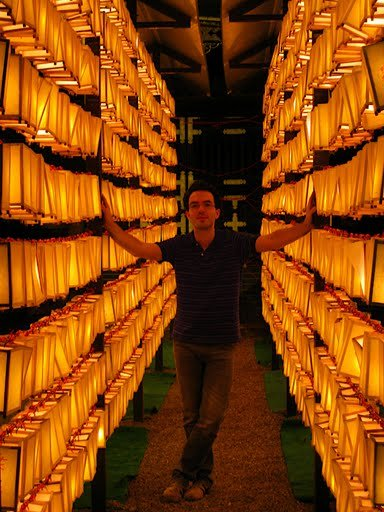
\includegraphics[height=0.3\textheight,clip=true,trim=3cm 7cm  2cm 5cm]{Mathieu}&
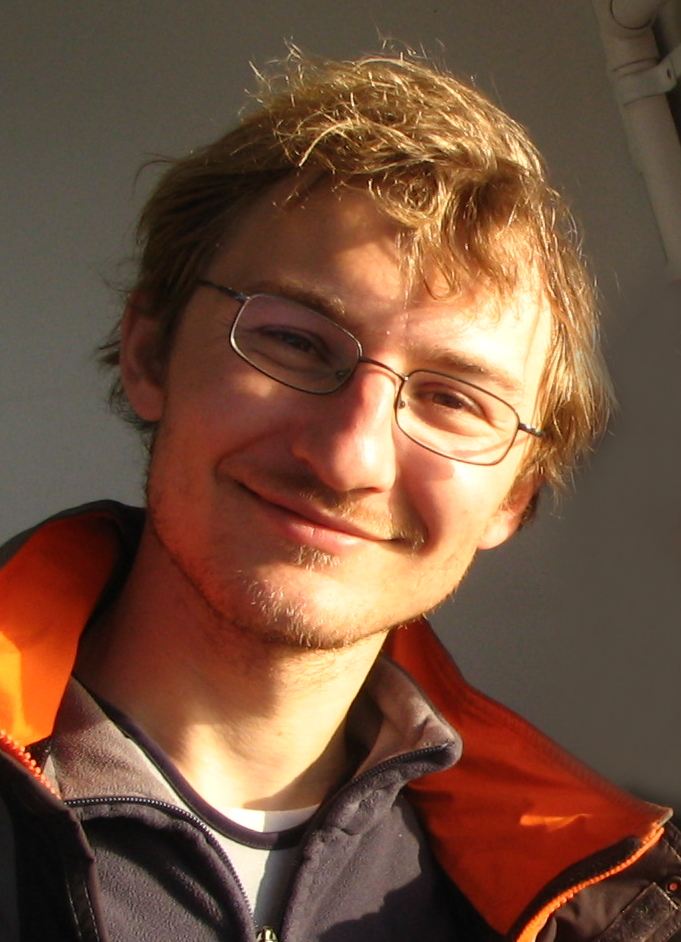
\includegraphics[height=0.3\textheight]{Thomas}&
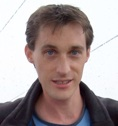
\includegraphics[height=0.3\textheight]{Seb}\\
Mathieu Nespoulous & Thomas Gibaud & Sebastien Manneville\\
Associate Professor & CNRS researcher & Professor\\
Aix-Marseille Université & E.N.S. Lyon & E.N.S. Lyon\\
\end{tabu}

\bigskip
\structure{Imaging plateform} BioSciences Gerland - Lyon Sud (UMS~3444)
\end{frame}

%\tikzset{external/force remake}
\begin{frame}{Over-acidification: Faster but weaker}
\begin{tikzpicture}
\begin{axis}[
	height=0.8\textheight,
	width=\textwidth,
	xlabel={time (h)}, ylabel={$G^\prime$ (\si{\pascal})},
	cycle list name=earthy,
	no marks,
	xmin=0, xmax=20,ymin=0,
	]
	\addplot table[x expr={\thisrowno{0}/3600}]{cas4_GDL1_Y265.prise} node[anchor=base west] {1\%};
	\addplot table[x expr={\thisrowno{0}/3600}]{cas4_GDL1.25_Y277.prise} node[anchor=base west] {1.25\%};
	\addplot table[x expr={\thisrowno{0}/3600}]{cas4_GDL1.5_Y275.prise} node[anchor=base west] {1.5\%};
	\addplot table[x expr={\thisrowno{0}/3600}]{cas4_GDL2_Y268.prise} node[anchor=base west] {2\%};
	\addplot table[x expr={\thisrowno{0}/3600}]{cas4_GDL3_Y270.prise} node[anchor=base west] {3\%};
	\addplot table[x expr={\thisrowno{0}/3600}]{cas4_GDL4_Y271.prise} node[anchor=base west, yshift=-0.2em] {4\%};
\end{axis}
\end{tikzpicture}

Caseins regain some solubility at low pH.
\end{frame}


\begin{frame}{Sealed cell, spontaneous pattern}
	
	\structure{Side view of the cell}\\
	\tikzsetnextfilename{cell_brushes}
	\tikzset{external/force remake}
	\begin{tikzpicture}[font=\footnotesize]
		\fill[pattern=north east lines,pattern color=Accent2] (0,0) rectangle (\textwidth,1.5em) node[midway,fill=white,inner sep=1pt] {glass};
		\fill[pattern=north east lines,pattern color=Accent2] (0,-2.5em) rectangle (\textwidth,-4em) node[midway,fill=white,inner sep=1pt] {glass};
		\draw[line width=2pt,Accent1] (0.05\textwidth,-2.5em) -- (0.95\textwidth,-2.5em) (0.05\textwidth,-1pt) -- (0.95\textwidth,-1pt) node[below,pos=0.30, text width=0.5\textwidth] {acrylamide brush ($10\sim 100$ nm)\linebreak $\Rightarrow$ No adhesion};
		\fill[gray] (0,0) rectangle (0.05\textwidth,-2.5em) (\textwidth,0) rectangle (0.95\textwidth,-2.5em) node[pos=1, above left] {spacer};
		\draw[<->] (0.75\textwidth,-2pt) -- (0.75\textwidth,-2.5em) node[midway,left] {$e\sim 100\,\mu m$};
		\draw[<->] (0.05\textwidth,2.25em) -- (0.95\textwidth,2.25em) node[midway,above] (L){$L\sim 2.5\,cm$};
		%\node[anchor=north west, inner sep=0] at ($(L.north) - (0.5\textwidth,0)$) {\structure{Side view of the cell}};
	\end{tikzpicture}
	
	\bigskip
	\structure{Top view of the final pattern}\\
	\begin{tikzpicture}[inner sep=0, very thick]
	\setlength{\mylength}{\columnwidth}
	\node[anchor=north west] (a) {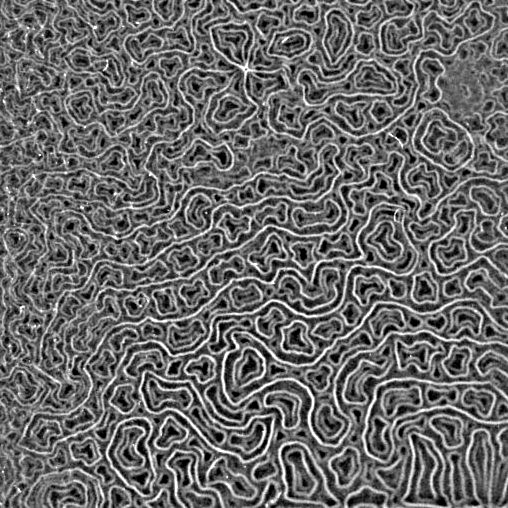
\includegraphics[width=0.28\mylength]{cas3p2_fluo0p8_GDL4_50um_coating_2_zoom2_crop}};
		\node[anchor=north] at (0.44\mylength,0) (b) {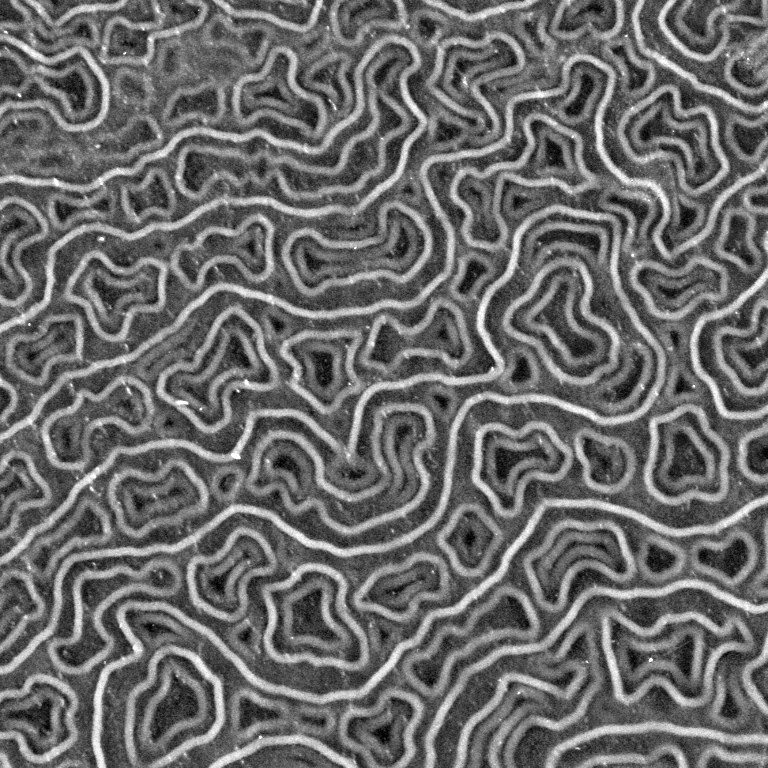
\includegraphics[width=0.28\mylength]{cas3p2_fluo0p8_GDL4_50um_coating_2_zoom6_crop}};
		\node[anchor=north east] at (\mylength,0) (c) {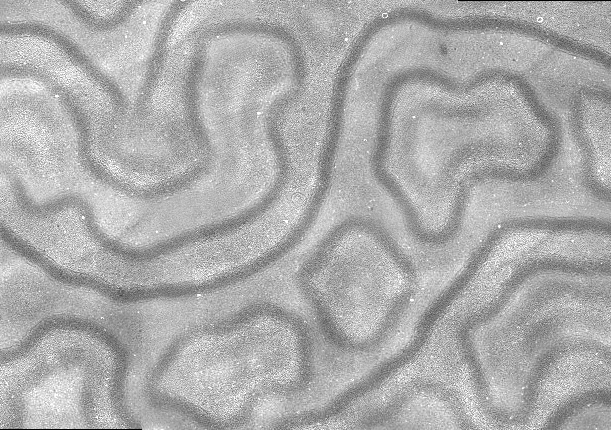
\includegraphics[width=0.4\mylength]{cas3p2_fluo0p8_GDL4_50um_coating_2_transmission}};
		%zooms
		\node[minimum width = 0.137\mylength, minimum height=0.137\mylength, anchor=north west, draw=Accent2] at ($(a.north west) +(0.111\mylength,-0.072\mylength)$) (bz){};
		\draw[Accent2] (bz.north east) -- (b.north west) (bz.south east) -- (b.south west);
		\node[minimum width = 0.128\mylength, minimum height=0.081\mylength, anchor=north west, draw=Main] at ($(b.north west) +(0.097\mylength,-0.143\mylength)$) (cz){};
		\draw[Main] (cz.north east) -- (c.north west) (cz.south east) -- (c.south west);
		\node[minimum width = 0.156\mylength, minimum height=0.156\mylength, anchor=north west, draw=Accent1] at ($(c.north west) + (0.125\mylength,0)$) (dz) {};
		%scale bars
		\draw[ultra thick] (a.south east) ++(0,-0.25em) -- ++(-0.178\mylength,0) node[pos=0.5, below=0.25em, font=\small] (M) {\SI{1}{\centi\metre}};
		\draw[ultra thick] (b.south east) ++(0,-0.25em) -- ++(-0.176\mylength,0) node[pos=0.5, below=0.25em, font=\small] {\SI{5}{\milli\metre}};
		\draw[ultra thick] (c.south east) ++(0,-0.25em) -- ++(-0.132\mylength,0) node[pos=0.5, below=0.25em, font=\small] {\SI{1}{\milli\metre}};
	\end{tikzpicture}
\end{frame}

\begin{frame}{Dynamics (transmission macroscope)}
\movie[externalviewer]{\begin{tikzpicture}
\node[inner sep=0] (a) {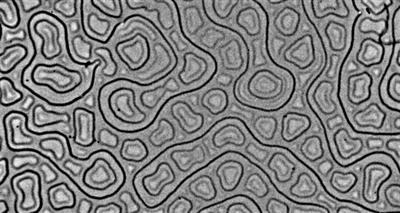
\includegraphics[width=\textwidth]{prise_0799_resized.jpg}};
\draw[line width=0.2em] ++(a.north west) -- ++(0.177\textwidth,0) node[pos=0, above right, inner xsep=0] {\SI{1}{\milli\metre}};
\end{tikzpicture}
}{cas4_GDL_4_100um_coat_macroscope_2.avi}
\end{frame}

\begin{frame}{Dynamics (transmission macroscope)}
\begin{tikzpicture}
	\matrix[matrix of nodes, inner sep=0, column sep=0.015\textwidth, row sep=0.5em, ampersand replacement=\&] (m){
	33 min \& 38 min \& 43 min \\
	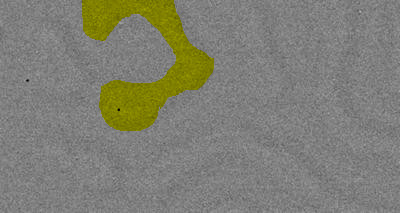
\includegraphics[width=0.32\textwidth]{prise_0100_color.jpg}\&
	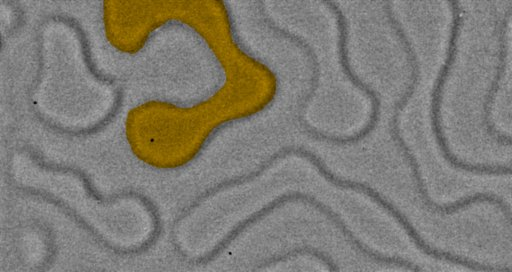
\includegraphics[width=0.32\textwidth]{prise_0130_color.jpg}\&
	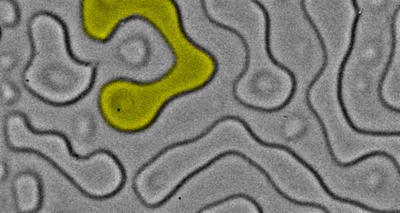
\includegraphics[width=0.32\textwidth]{prise_0160_color.jpg}\\
	48 min \& 1h \& 1h15 \\
	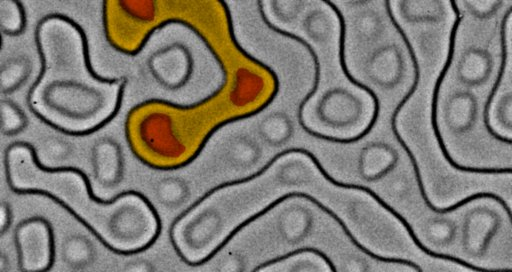
\includegraphics[width=0.32\textwidth]{prise_0190_color.jpg}\&
	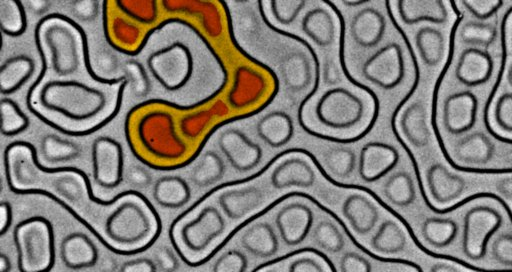
\includegraphics[width=0.32\textwidth]{prise_0250_color.jpg}\&
	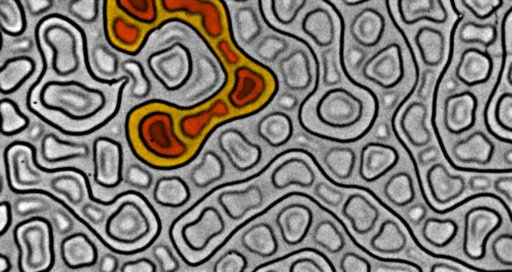
\includegraphics[width=0.32\textwidth]{prise_0360_color.jpg}\\
	};
	\draw[line width=0.2em] ++(m-4-1.south west) -- ++(0.056\textwidth,0) node[pos=0, below right, inner xsep=0] {\SI{1}{\milli\metre}};
\end{tikzpicture}

\begin{itemize}
\item nesting patterns
\item length scale becomes smaller
\end{itemize}
\end{frame}

\begin{frame}{What is going on in the thickness?}
\begin{columns}
\column{0.4\textwidth}
\begin{itemize}
\item fluorescent casein
\item confocal microscope
\item[$\Rightarrow$] 3D concentration field
\end{itemize}

\begin{tikzpicture}
\draw[ultra thick] (0,) -- +(0.786\textwidth,0) node[midway, above] {\SI{1}{\milli\metre}};
\end{tikzpicture}
\setlength{\tabcolsep}{1pt}
\begin{tabular}{p{\columnwidth}l}
	
\includegraphics[width=\columnwidth, height=0.061\columnwidth]{coupe_cloque_t000.png}& \SI{15}{\minute}\\
	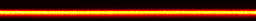
\includegraphics[width=\columnwidth, height=0.061\columnwidth]{coupe_cloque_t011.png} & \SI{22}{\minute}\\
	\includegraphics[width=\columnwidth, height=0.061\columnwidth]{coupe_cloque_t110.png} & \SI{1}{\hour}~26\onslide<2->{\\
	\includegraphics[width=\columnwidth, height=0.061\columnwidth]{coupe_cloque_t116.png} & \SI{1}{\hour}~30\\
	\includegraphics[width=\columnwidth, height=0.061\columnwidth]{coupe_cloque_t117.png} & \SI{1}{\hour}~31\\
	\includegraphics[width=\columnwidth, height=0.061\columnwidth]{coupe_cloque_t123.png} & \SI{1}{\hour}~35\\
	\includegraphics[width=\columnwidth, height=0.061\columnwidth]{coupe_cloque_t200.png} & \SI{2}{\hour}~25\\
	\includegraphics[width=\columnwidth, height=0.061\columnwidth]{coupe_cloque_t221.png} & \SI{2}{\hour}~40\\}
\end{tabular}

\begin{itemize}
\item synæresis and swelling
\item<2-> cause buckling
\end{itemize}
\column{0.1\textwidth}

\column{0.5\textwidth}
\begin{tikzpicture}
	\begin{groupplot}[%
		group style={
			group name=g, group size=1 by 3,
			xticklabels at=edge bottom,
			vertical sep=0,
			},
		xmin=0, xmax=170, xtick={0,30,...,150},
		extra tick style={grid=major},%
		extra x ticks = {21,68}, extra x tick labels={},%
		scale only axis,
		width=\textwidth-4em,
		height=5\baselineskip,
		ylabel absolute, every axis y label/.append style={anchor=base, yshift=-1em}
		]
	\nextgroupplot[
		ylabel={$G^\prime$ (\si{\pascal})},
		ymin=0,
		]
	\addplot+[no marks,Accent1] table[x expr={\thisrowno{0}/60}]{cas4_GDL4_Y271.prise};
	\node[below left] at (rel axis cs:1,1) {rheometer (stick)};
	
	\nextgroupplot[
		ylabel={Volume (\%)}, ymin=20, ymax=100, 
		ytick={40,60,80,100}, every axis y label/.append style={xshift=0.5em},
		]
	\addplot+[no marks,Accent1] table[x expr={\thisrowno{0}+15}, y expr={\thisrowno{1}*100}]{relative_volume_excess_area_cloques.txt};
	%\addplot+[only marks,Accent2, mark=+] table[y expr={\thisrowno{1}*100}]{volume_rel_half_cas8_toi.txt};
	\node[anchor=south west] at (rel axis cs:0,0) {\rotatebox{90}{synæresis}};
	\node at (axis cs:68,80) {swelling};
	
	\nextgroupplot[
		ylabel={Excess area (\%)}, ymin=0, ymax=4, ytick={0,1,2,3},
		xlabel={time (min)}, 
		every axis y label/.append style={xshift=-1em},
		]
	\only<2->{\addplot+[no marks,Accent1] table[x expr={\thisrowno{0}+15}, y expr={\thisrowno{2}*100}]{relative_volume_excess_area_cloques.txt} node[pos=1, below left] {all};
	\addplot+[no marks,Accent2] table[x expr={\thisrowno{0}+15}, y expr={\thisrowno{3}*100}]{relative_volume_excess_area_cloques.txt} node[pos=1, left] {single blister};
	\draw[->] (axis cs: 21, 3) -- (axis cs: 68, 3) node[midway, below] {\SI{1}{\hour}};}
	%\legend{all, single blister};
	\end{groupplot}
	\end{tikzpicture}
\end{columns}
\end{frame}

\begin{frame}{Dynamics (confocal microscope)}
\movie[externalviewer]{\begin{tikzpicture}
	\node[inner sep=0] (a) {\includegraphics[width=\textwidth]{cas3p2_fluo0p8_GDL4_2_t260_crop_resized.jpg}};
	\draw[line width=0.2em] ++(a.south west) -- ++(0.75\textwidth,0) node[pos=0, below right, inner xsep=0] {\SI{1}{\milli\metre}};
	
	\node[above=1em of a, inner sep=0] (c) {\includegraphics[width=0.4\textwidth]{cas3p2_fluo0p8_GDL4_50um_coating_2_transmission}};

	\node[minimum width = 0.156\textwidth, minimum height=0.156\textwidth, anchor=north west, draw=Accent1] at ($(c.north west) + (0.125\textwidth,0)$) (dz) {};
	\draw[ultra thick] (c.south east) ++(0,-0.25em) -- ++(-0.132\textwidth,0) node[pos=0.5, below=0.25em, font=\small] {\SI{1}{\milli\metre}};
\end{tikzpicture}
}{volume_plis.avi}
\end{frame}

\begin{frame}{Dynamics (confocal microscope)}
\begin{tikzpicture}
	\matrix[matrix of nodes, inner sep=0, column sep=0.015\textwidth, row sep=0.5em, ampersand replacement=\&] (m){
	33 min \& 38 min \& 43 min \\
	\includegraphics[width=0.32\textwidth]{cas3p2_fluo0p8_GDL4_2_t047_crop_resized.jpg}\&
	\includegraphics[width=0.32\textwidth]{cas3p2_fluo0p8_GDL4_2_t056_crop_resized.jpg}\&
	\includegraphics[width=0.32\textwidth]{cas3p2_fluo0p8_GDL4_2_t065_crop_resized.jpg}\\
	48 min \& 1h \& 1h15 \\
	\includegraphics[width=0.32\textwidth]{cas3p2_fluo0p8_GDL4_2_t074_crop_resized.jpg}\&
	\includegraphics[width=0.32\textwidth]{cas3p2_fluo0p8_GDL4_2_t092_crop_resized.jpg}\&
	\includegraphics[width=0.32\textwidth]{cas3p2_fluo0p8_GDL4_2_t125_crop_resized.jpg}\\
	};
	\draw[line width=0.2em] ++(m-4-1.south west) -- ++(0.24\textwidth,0) node[pos=0, below right, inner xsep=0] {\SI{1}{\milli\metre}};
\end{tikzpicture}

\begin{columns}
\column{0.32\textwidth}
\begin{itemize}
\item confinement
\item cascade buckling
\item wavelength division
\end{itemize}
\column{0.68\textwidth}
\includegraphics[width=\columnwidth]{Roman_1999_confined.jpg}

\textit{\footnotesize Roman \& Pocheau, EPL (1999)}
\end{columns}

\begin{center}
\alert{Where does the initial wavelength come from?}
\end{center}
\end{frame}


\begin{frame}<1-2>[label=carpet]{Wavelength: resisting stress needed}
\structure{Simple case} Initial flat contact with the substrate: carpet
\begin{columns}
\column{0.5\textwidth}
\temporal<2>{
	\includegraphics[width=\columnwidth, height=0.061\columnwidth]{coupe_cloque_t000.png}\\
	\includegraphics[width=\columnwidth, height=0.061\columnwidth]{coupe_cloque_t011.png}\\
	\includegraphics[width=\columnwidth, height=0.061\columnwidth]{coupe_cloque_t110.png}\\
	\includegraphics[width=\columnwidth, height=0.061\columnwidth]{coupe_cloque_t116.png}\\
	\includegraphics[width=\columnwidth, height=0.061\columnwidth]{coupe_cloque_t117.png}\\

	\includegraphics[width=\textwidth]{volume_cloque_t116}\\
	\begin{tikzpicture}
	\draw[ultra thick] (0,) -- +(0.786\textwidth,0) node[midway, below] {\SI{1}{\milli\metre}};
	\end{tikzpicture}
	
	\structure{In our case}
	\begin{itemize}
	\item Vertical cells show the same wavelength
	\item $\sigma \neq \rho g h$
	\end{itemize}
}{

\bigskip
\begin{itemize}
\item solvent must flow through gel
\begin{description}[$\ell_p$]
\item[$v$] gel velocity = -volumic flux $\simeq \SI{0.2}{\micro\metre\per\second}$
\item[$\ell_p$] pore size $ \approx \SI{4}{\micro\metre}$
\end{description}
\item $\sigma$ is a Darcy pressure
\[\sigma = \Delta P \sim \eta h v/\ell_p^2\]
\item poroelastic length
\[ \lambda^* \sim \left(\frac{B \ell_p^2}{\eta v h}\right)^\frac{1}{3} \simeq \SI{2}{\milli\metre}\]
\end{itemize}
}{
\begin{tikzpicture}
\begin{axis}[
	width=\textwidth,
	height=0.6\textwidth,
	xmin=0, xmax=1000, xtick={0,250, 500, 750}, xlabel={position (\si{\micro\metre})},
	ymin=0, ymax=50, ylabel={altitude (\si{\micro\metre})},
	cycle list name=earthy,
	no marks,
	]
	\draw[ultra thick, Accent2] (axis cs:580,0) -- (axis cs:580,50);
	\foreach \x in {2,3,..., 8}
		\addplot table[y index=\x]{alts_bottom_cloque.txt};
\end{axis}
\end{tikzpicture}
\begin{itemize}
\item $\lambda$ frozen at ceiling touch 
\item $A=H\equiv e-h$
\item $\lambda \sim \epsilon^{-3/7} H \sim e$
	%\[ \epsilon \sim \left(\frac{\lambda}{e}\frac{e}{H}\right)^{-7/3} \simeq 0.6\% \]
\end{itemize}
}

\column{0.5\textwidth}
\begin{block}{Ruck in a rug}
\begin{tikzpicture}[ultra thick]
\begin{axis}[
	name=a,
	width=\textwidth, height=3\baselineskip, scale only axis,
	domain=-180:180, no markers, ymin=0, ymax=3,xmin=-180,xmax=180,
	axis lines=none, xtick=\empty,
	axis background/.style={fill=white},
	]
	\addplot+[Accent1]{cos(x)+1};
	\addplot+[Accent1]{cos(x)+1.5};
	\draw[->, Accent2, ultra thick] (axis cs:90,1.25) -- (axis cs:90,2.25) node[pos=1, right] {$v$};
	\draw[Main, ultra thick, {Circle}->] (axis cs:-90,1.5) -- (axis cs:-90,0.25) node[right] {$\sigma$};
	%\node[above] at (axis cs:-90,1.5) {$P_2$};
	%\node[below right] at (axis cs:-90,1.25) {$P_1$};
	\draw[<->, ultra thick] (axis cs:0,0) -- (axis cs:0,2) node[midway, right] {$A$};
	\draw[<->] (axis cs:0,2) -- (axis cs:0,2.5) node[midway, right] {$h$};
\end{axis}
\fill[pattern=north east lines,pattern color=Accent2] (a.south west) rectangle ($(a.south east)+(0,-1em)$);
\draw[<->] ($(a.south west)+(0,-1.1em)$) -- ($(a.south east)+(0,-1.1em)$) node[midway, below] {$\lambda$};
\end{tikzpicture}

\textit{\footnotesize Kolinski et al., Vella et al. PRL 2009}\\
\begin{description}[$B$]
\item[$\epsilon$] excess area \hfill$\Rightarrow$ buckling 
\item[$B$] bending modulus \hfill$\Rightarrow \lambda\nearrow$
\item[$\sigma$] vertical stress \hfill$\Rightarrow \lambda\searrow$
\end{description}
\[ \lambda^* \equiv \left(\frac{B}{\sigma}\right)^{1/3}\text{, eg. }\sigma =\rho g h \]
$\lambda \sim \epsilon^{1/7} \lambda^*$ and $A \sim \epsilon^{4/7} \lambda^*$
\end{block}
\end{columns}
\end{frame}

\begin{frame}{Poroelasticity}
\begin{columns}\column{0.15\textwidth}
\includegraphics[width=\textwidth]{Henry_Darcy}
\column{0.85\textwidth}
\begin{block}{Henry Darcy (1803-1858)}
\begin{description}[1803]
\item[1846] granted lifelong free water
\item[1856] \textit{Les fontaines publiques de la ville de Dijon}
\end{description}
\end{block}
\end{columns}

\begin{columns}
\column{0.15\textwidth}
\includegraphics[width=\textwidth]{Maurice_Anthony_Biot}
\column{0.58\textwidth}
\begin{block}{Maurice Anthony Biot (1905-1985)}
\begin{description}[1803]
%\item[1932] Ph.D. under von Kármán (Cal Tech)
\item[1932-1942] earthquake engineering
\item[1935-1962] theory of poroelasticity
\end{description}
\end{block}
\column{0.27\textwidth}
\includegraphics[width=\textwidth]{Biot_1964_Buckling_Porous}
\end{columns}

\medskip
\begin{footnotesize}
\textit{Biot, J. Appl. Mech. 1964}: Buckling of a porous slab embedded in an impervious infinite viscous or viscoelastic medium
\end{footnotesize}
\begin{itemize}
\item $B$ transiently higher due to pore pressure
\item $\sigma$ comes only from the surrounding medium $\rightarrow 0$
\item effect of flow through the porous slab not considered
\end{itemize}
\end{frame}

\begin{frame}{No initial contact with a substrate}
\structure{Poiseuille vs Darcy on a flying carpet}
\begin{tikzpicture}
\begin{axis}[
	name=a,
	width=\textwidth, height=0.25\textwidth, scale only axis,
	domain=0:360, no markers, ymin=-4, ymax=4,xmin=0,xmax=360,
	axis lines=none, xtick=\empty,
	]
	\fill[gray!20] (axis cs:85,4) rectangle (axis cs:95,-4) (axis cs:265,4) rectangle (axis cs:275,-4);
	\addplot+[Accent1]{sin(x)+0.5};
	\addplot+[Accent1]{sin(x)-0.5};
	\addplot+[dashed, black]{0.5};
	\addplot+[dashed, black]{-0.5};
	\draw[<->, help lines] (axis cs:180,0.5) -- (axis cs:180,4) node[midway, left] {$H$}; 
	\draw[<->, help lines] (axis cs:30,-0.5) -- (axis cs:30,-4) node[midway, left] {$H$};
	\node[below] at (axis cs:90,-1.5) (pb1) {$P_1$};
	\node[above] at (axis cs:90,1.5) (ph2) {$P_2$};
	\node[above] at (axis cs:270,1.5) (ph1) {$P_1$};
	\node[below] at (axis cs:270,-1.5) (pb2) {$P_2$};
	\draw[line width=0.1em, ->] (ph2) -- (axis cs:90,0.5) node[midway, left] {Darcy} node[midway, right] {$v$};
	\draw[line width=0.1em, ->] (pb2) -- (pb1) node[midway, above] {Poiseuille} node[midway, below] {$u \sim \frac{\lambda}{H} v$};
\end{axis}
\fill[pattern=north east lines,pattern color=Accent2] (a.south west) rectangle +(\textwidth,-1em) (a.north west) rectangle +(\textwidth,1em);
\end{tikzpicture}

\begin{columns}
\column{0.83\textwidth}
\begin{itemize}
\item The same $\Delta P$ can be relaxed by a Poiseuille flow
\[\Delta P \sim 12\eta\frac{\lambda}{H^2} u \sim 12\eta\frac{\lambda^2}{H^3} v\]
\item For the same wavelength
\hfill$\displaystyle \frac{v_\text{Darcy}}{v_\text{Poiseuille}} \sim \frac{\ell_p^2\lambda^2}{hH^3} \approx 30$
\item Flow through the pores dominates
\end{itemize}
\column{0.17\textwidth}
\includegraphics[width=\textwidth]{Jean-Leonard-Marie_Poiseuille.jpg}\\
\hfill\structure{1797-1869}
\end{columns}
\end{frame}

\againframe<3>{carpet}

\end{document}

